% LaTeX Template
% Version 1.3 (21/12/12)
%
% This template has been downloaded from:
% http://www.latextemplates.com
%
% Original authors:
% Steven Gunn 
% http://users.ecs.soton.ac.uk/srg/softwaretools/document/templates/
% and
% Sunil Patel
% http://www.sunilpatel.co.uk/thesis-template/
%
% License:
% CC BY-NC-SA 3.0 (http://creativecommons.org/licenses/by-nc-sa/3.0/)
%
% Note:
% Make sure to edit document variables in the Thesis.cls file
%
%%%%%%%%%%%%%%%%%%%%%%%%%%%%%%%%%%%%%%%%%

%----------------------------------------------------------------------------------------
%	PACKAGES AND OTHER DOCUMENT CONFIGURATIONS
%----------------------------------------------------------------------------------------

\documentclass[11pt, a4paper, oneside]{Thesis} % Paper size, default font size and one-sided paper

\usepackage[utf8]{inputenc}
\usepackage[section]{placeins}


\graphicspath{{./Pictures/}} % Specifies the directory where pictures are stored

\usepackage[square, numbers, comma, sort&compress]{natbib} % Use the natbib reference package - read up on this to edit the reference style; if you want text (e.g. Smith et al., 2012) for the in-text references (instead of numbers), remove 'numbers' 
\hypersetup{urlcolor=blue, colorlinks=true} % Colors hyperlinks in blue - change to black if annoying
\title{\ttitle} % Defines the thesis title - don't touch this

\begin{document}

\frontmatter % Use roman page numbering style (i, ii, iii, iv...) for the pre-content pages

\setstretch{1.3} % Line spacing of 1.3

% Define the page headers using the FancyHdr package and set up for one-sided printing
\fancyhead{} % Clears all page headers and footers
\rhead{\thepage} % Sets the right side header to show the page number
\lhead{} % Clears the left side page header

\pagestyle{fancy} % Finally, use the "fancy" page style to implement the FancyHdr headers

\newcommand{\HRule}{\rule{\linewidth}{0.5mm}} % New command to make the lines in the title page

% PDF meta-data
\hypersetup{pdftitle={\ttitle}}
\hypersetup{pdfsubject=\subjectname}
\hypersetup{pdfauthor=\authornames}
\hypersetup{pdfkeywords=\keywordnames}

%----------------------------------------------------------------------------------------
%	TITLE PAGE
%----------------------------------------------------------------------------------------

\begin{titlepage}
\begin{center}

\textsc{\LARGE \univname}\\[1.5cm] % University name
\textsc{\Large Memoria Titulación}\\[0.5cm] % Thesis type

\HRule \\[0.4cm] % Horizontal line
{\huge \bfseries \ttitle}\\[0.4cm] % Thesis title
\HRule \\[1.5cm] % Horizontal line
 
\begin{minipage}{0.4\textwidth}
\begin{flushleft} \large
\emph{Autor:}\\
\end{flushleft}
\end{minipage}
\begin{minipage}{0.4\textwidth}
\begin{flushright} \large
\emph{Supervisores:} \\
\end{flushright}
\end{minipage}\\[3cm]
 
\large \textit{Memoria para optar al grado de \degreename}\\[0.3cm] % University requirement text
\textit{en el}\\[0.4cm]
\deptname\\[2cm] % Research group name and department name
 
{\large \today}\\[4cm] % Date
%\includegraphics{Logo} % University/department logo - uncomment to place it
 
\vfill
\end{center}

\end{titlepage}

%----------------------------------------------------------------------------------------
%	DECLARATION PAGE
%	Your institution may give you a different text to place here
%----------------------------------------------------------------------------------------



%----------------------------------------------------------------------------------------
%	QUOTATION PAGE
%----------------------------------------------------------------------------------------



%----------------------------------------------------------------------------------------
%	ABSTRACT PAGE
%----------------------------------------------------------------------------------------

\addtotoc{Abstract} % Add the "Abstract" page entry to the Contents

\abstract{\addtocontents{toc}{\vspace{1em}} % Add a gap in the Contents, for aesthetics
Desarrollo de una plataforma, de bajo costo, que permita estudiar el comportamiento de grupos de robots. Para que la plataforma funcione es necesario el diseño y construcción de los robots , implementar sistema de tracking 2D, armar la red de comunicación (XBee) y construir el software de control.
}

\clearpage % Start a new page


%----------------------------------------------------------------------------------------
%	ACKNOWLEDGEMENTS
%----------------------------------------------------------------------------------------

\setstretch{1.3} % Reset the line-spacing to 1.3 for body text (if it has changed)

\acknowledgements{\addtocontents{toc}{\vspace{1em}} % Add a gap in the Contents, for aesthetics 

Este trabajo no habría podido realizarse sin el apoyo incondicional de mi profesora tutora, Dra. María José Escobar que ha tenido una paciencia infinita conmigo y siempre me ha ayudado en lo posible. También fue fundamental el apoyo del Dr. Juan Cristóbal Zagal que gentilmente me permitió trabajar en su innovador laboratorio de Síntesis de máquinas inteligentes. No menos importante fue el apoyo del Dr. Pablo Prieto que ha sido un guía para mí en el diseño del robot. Además de ellos conté con la ayuda de mucha gente que sea han dedicado a escuchar mis ideas y aconsejarme. Es por esto que quiero agradecer a Jaime Martínez por ayudarme a diseñar el PCB de MODI, Carlos Galáz por sus infinitos minutos telefónicos para discutir casi todos los aspectos de MODI, Fabián Rubilar por sus ideas de como mover los robots, Linus Casassa por su paciencia para explicarme cualquier cosa sobre electrónica, la gente del taller de electrónica por enseñarme a soldar y sacarme de apuros técnicos, Ricardo Pérez por las interminables discusiones sobre el robot, mis compañeros del laboratorio de Sintesís de máquinas inteligentes y a mi amada Pía que siempre ha estado ahí conmigo siendo un gran apoyo en mi vida.
}
\clearpage % Start a new page

%----------------------------------------------------------------------------------------
%	LIST OF CONTENTS/FIGURES/TABLES PAGES
%----------------------------------------------------------------------------------------

\pagestyle{fancy} % The page style headers have been "empty" all this time, now use the "fancy" headers as defined before to bring them back

\lhead{\emph{Contents}} % Set the left side page header to "Contents"
\tableofcontents % Write out the Table of Contents

\lhead{\emph{Índice de Figuras y Tablas}} % Set the left side page header to "List of Figures"
\listoffigures % Write out the List of Figures


%----------------------------------------------------------------------------------------
%	DEDICATION
%----------------------------------------------------------------------------------------

\setstretch{1.3} % Return the line spacing back to 1.3

\pagestyle{empty} % Page style needs to be empty for this page

\dedicatory{Pía, mi fiel compañera de aventuras\ldots} % Dedication text

\addtocontents{toc}{\vspace{2em}} % Add a gap in the Contents, for aesthetics

%----------------------------------------------------------------------------------------
%	THESIS CONTENT - CHAPTERS
%----------------------------------------------------------------------------------------

\mainmatter % Begin numeric (1,2,3...) page numbering

\pagestyle{fancy} % Return the page headers back to the "fancy" style

% Include the chapters of the thesis as separate files from the Chapters folder
% Uncomment the lines as you write the chapters

% Chapter 1

\chapter{Introducción} % Introduccion al trabajo

\label{Chapter1} % For referencing the chapter elsewhere, use \ref{Chapter1} 

\lhead{Capítulo 1. \emph{Introducción}} % This is for the header on each page - perhaps a shortened title

%----------------------------------------------------------------------------------------

%--------------------------------------------------------
%Sección 1
%--------------------------------------------------------


\begin{figure}[htbp]
	\centering
		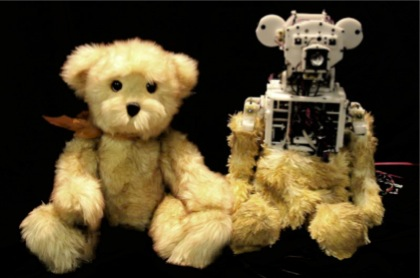
\includegraphics[width=0.8\textwidth]{./Figures/robot.jpg}
		%\rule{35em}{0.5pt}
%	\caption[Robot Huggable]{Robot creado por MIT Media Lab para cuidados personales. Imagen tomada de \cite{Stiehl:2006:HTR:1179133.1179149}}
	\label{fig:Huggable}
\end{figure}

El trabajo se centró en la investigación de las tecnologías existente para diseñar un robot que sea económico, simple y que de manera inalámbrica permita su control. El robot debe tener estas características ya que se necesita construir un enjambre para poder realizar estudios en el comportamiento y control de estos.

Al comienzo de este proyecto se trabajó en Santiago de Chile, en conjunto con la Universidad de Chile (UChile) bajo la tutela del Doctor Juan Cristóbal Zagal en el Laboratorio de Síntesis de Máquinas Inteligentes. Por parte de la Universidad Técnica Federico Santa María (USM), se trabajó con la Doctora María José Escobar, del Departamento de Electrónica y luego se incorporó el Doctor Pablo Prieto del Departamento de Diseño de Productos. El financiamiento para realizar este prototipo ha sido por parte de las dos Instituciones, Universidad Técnica Federico Santa María y Universidad de Chile.

Durante el proceso de desarrollo se tuvieron que hacer diversas compras de materiales, pero los lugares más recurrentes al momento de hacerlas fueron Olimex y Casa Royal. La primera es una empresa dedicada a traer productos para hacer prototipos y construir máquinas, la segunda cuenta con varios insumos básicos para trabajar en desarrollo de circuitos electrónicos. Ambas empresas se encuentran en Santiago, por lo que trabajar en esta ciudad es de gran ayuda para reducir los tiempos en desarrollo.
Luego de armar un primer robot funcional, con materiales disponibles en Santiago de Chile, se hizo una búsqueda en internet de componentes en tiendas especializadas.

Este documento resume el desarrollo del proyecto MODI (Modular Intelligent), que es un robot simple de construir que tiene como fin ser repetible para facilitar la construcción de Enjambres de robots. El capítulo 2 se explica lo que es un robot, algo de historia y algunos tipos de robots. El capítulo 3 comienza con un explicación sobre los enjambres de animales, luego se describen los robots usados actualmente en la literatura para estudiar enjambres y al final se describe las necesidades de mercado y las ventajas del proyecto MODI. El capítulo 4 está centrado en el diseño y herramientas de fabricación utilizadas durante el proceso de desarrollo. El capítulo 5 es el principal, describe criterios de diseño y el detalle de todos los componentes utilizados en el robot diseñado. Además se explica el software utilizado y el sistema que permite hacer un seguimiento de cada robot de forma individual. En el capítulo 6 se explican algunos posibles usos de los enjambres de robots. Al final, el capítulo 7 tiene sugerencias para mejoras futuras y las conclusiones.

%---------------------------------------------------------------------------------------- 
% Chapter Template

\chapter{Swarm} % Main chapter title

\label{Chapter2} % Change X to a consecutive number; for referencing this chapter elsewhere, use \ref{ChapterX}

\lhead{Capítulo 2. \emph{Swarms}} % Change X to a consecutive number; this is for the header on each page - perhaps a shortened title

%----------------------------------------------------------------------------------------
%	SECTION 1
%----------------------------------------------------------------------------------------

\section{Comportamiento colectivo en la naturaleza}

\begin{figure}[htbp]
	\centering
		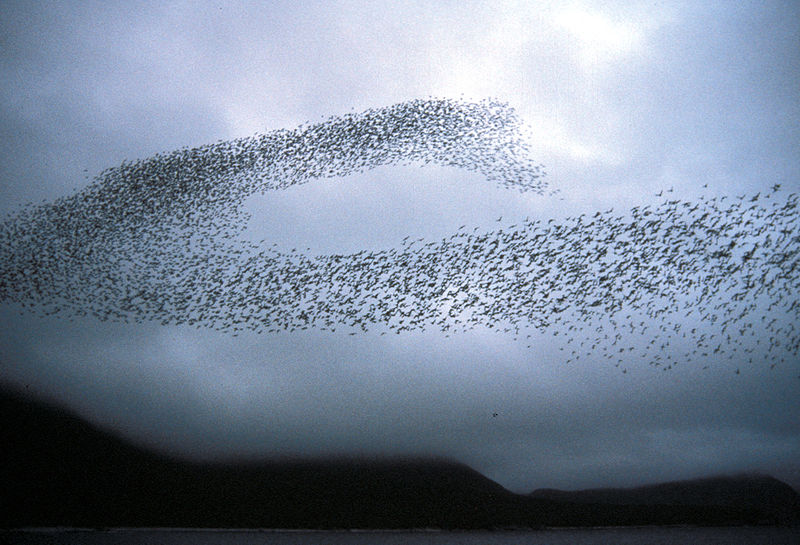
\includegraphics[width=0.8\textwidth]{./Figures/swarm.jpg}
		\rule{35em}{0.5pt}
	\caption[swarm]{Bandada de auklets, teniendo comportamiento de enjambre. Imagen extraida de Wikipedia.}
	\label{fig:swarm}
\end{figure}

Existen casos de enjambres, los más típicos son las hormigas y abejas, pero los hay en peches, aves e incluso los mamíferos. Son sistemas donde nadie está a cargo y aún así ejecutan una tarea grupal. Las hormigas son un gran ejemplo. Al momento de construir su nido, no tienen un arquitecto o ingeniero estructural que esté dando órdenes, simplemente cada una sabe que tiene que hacer. No hay un director orquestando la construcción desde lo alto, en vez de esto lo que ocurre es un comportamiento emergente. También conocido como inteligencia de enjambre.

Otro tipo de comportamiento colectivo son las migraciones, desplazamientos periódicos que efectúan aves, peces, langostas y mamíferos de un hábitat a otro. Cada individuo activo en la migración sigue al grupo, los más pequeños como el plancton o anfibios aprovechan las corrientes de aire o agua, y las aves, más grandes, aprovechan los vientos y corrientes ascendentes. Hay diversas finalidades detrás de la migración, algunas especies lo hacer para escaparse de los crudos inviernos o secos veranos; mientras que otras, como las tortugas marinas, por una necesidad reproductiva emprenden un largo viaje de más de 10.000 millas, a lo largo de todo el Atlántico Norte.

Lograr que un enjambre de robots tenga un comportamiento emergente como el de las colonias de abejas es la piedra filosofal de los investigadores de esta área. Uno de los más destacados investigadores del área, James McLurkin, experto en robótica del Massachusetts Institute of Technology (MIT) dice que para lograrlo es necesario un software que ejecute tareas individuales y     que de alguna forma se cumpla con una tarea grupal. He aquí una importante razón para desarrollar estudios sobre enjambres de robots, ya que aún no está claro cómo se coordina la naturaleza para llevar a cabo tales tareas.

%-----------------------------------
%	SECTION 2
%-----------------------------------
\section{Robots para construir un enjambre}

Imaginemos una situación hipotética donde un edificio es destruido, la búsqueda de sobrevivientes no es una tarea fácil, implica que rescatistas ingresen al lugar corriendo grave peligro, usualmente buscando a las víctimas en condiciones de poca visibilidad. Esto mismo podría ser ejecutado por un enjambre robótico que esté programado para buscar gente y que de manera colectiva recorra un área mucho mayor que 2 o 3 personas. Incluso un robot del mismo enjambre puede fallar, pero al ser un sistema distribuido el enjambre continúa funcionando, es un sistema muy robusto.

A continuación algunos robots que pueden ser utilizados para hacer un Robot Swarm junto con las información técnica disponible.

%-----------------------------------
%	SUBSECTION 1
%-----------------------------------

\subsection{Kilobot}
El proyecto Kilobot, es un sistema de bajo costo escalable para demostrar comportamientos colectivos. Actualmente existen varios grupos que están investigando algoritmos para enjambres de robots, por esto que diseñaron Kilobot que es un robot de bajo costo, accesible,  que permite hacer pruebas en cientos o miles de robots.

\begin{figure}[htbp]
	\centering
		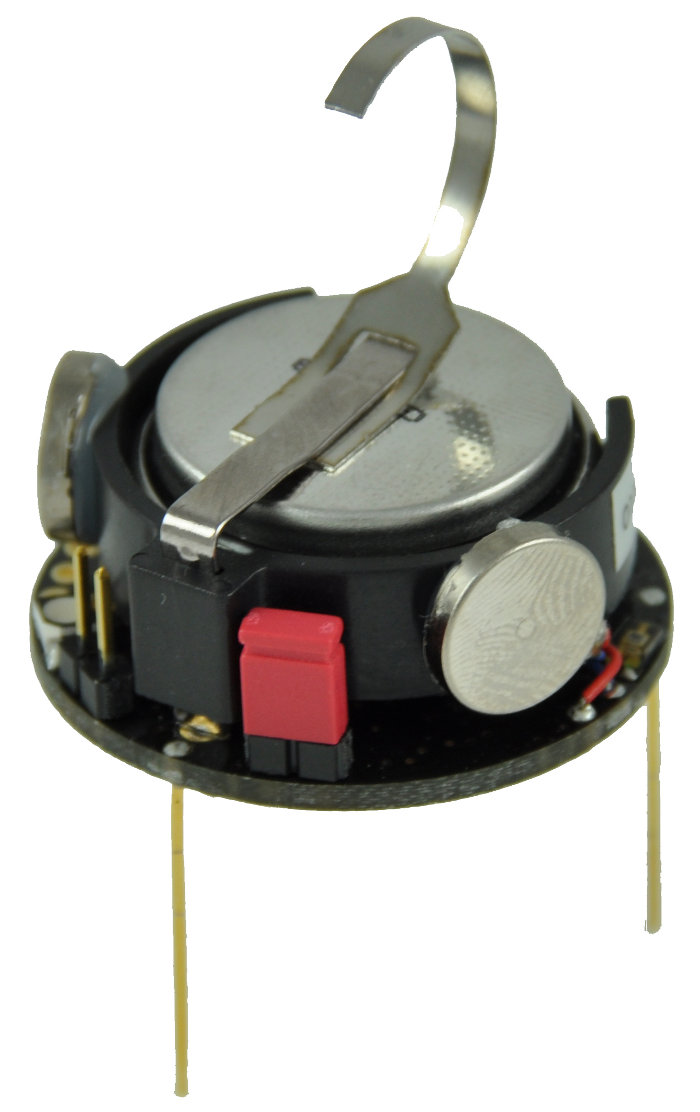
\includegraphics[width=0.4\textwidth]{./Figures/kilobot.jpg}
		\rule{35em}{0.5pt}
	\caption[swarm]{Kilobot. Imagen extraida de http://www.k-team.com.}
	\label{fig:kilobot}
\end{figure}



%-----------------------------------
%	SUBSECTION 2
%-----------------------------------

\subsection{Organismo Multibot}

S. Kornienko, O. Kornienko, A. Nagarathinam y P. Levi., exploran el trabajo colaborativo en robots para un mejor rendimiento y mayor fiabilidad a nivel macroscopico. En este articulo demuestran sus últimos trabajos en sistemas colectivos y lo más sorprendente es que logran la agregación y desagregación autónoma para así obtener un organismo multibot.
\cite{5359578}

\begin{figure}[htbp]
	\centering
		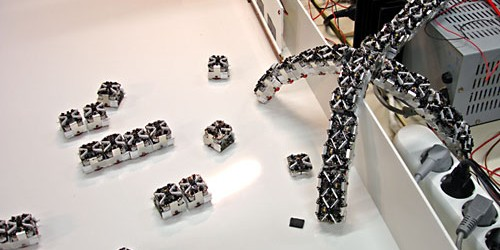
\includegraphics[width=0.7\textwidth]{./Figures/Multibot_organism.jpg}
		\rule{35em}{0.5pt}
	\caption[swarm]{Organismo Multibot. Imagen extraida de http://ieeesbcet.org/}
	\label{fig:Organismo}
\end{figure}


%-----------------------------------
%	SUBSECTION 3
%-----------------------------------

\subsection{E-puck}

Uno de los robots más utilizados por los científicos en el mundo para estudios y publicaciones es el E-puck. Este robot es compacto, tiene forma de cilindro con un diámetro de 7 [cm] y para moverse hace uso de sus dos ruedas, dejándolo en la categoría de robot con desplazamiento diferencial. Originalmente fue diseñado para educar en el área de la micro ingeniería por Michael Bonani y Francesco Mondala en el laboratorio ASL del Profesor Roland Siegwart en Escuela Politécnica Federal de Lausana (EPFL) en Suiza. El e-puck es open hardware, software es de código abierto,  lo construyen y venden varias empresas. Para comunicarse con una computador incorporan un módulo Bluetooth conectado a uno de sus dos puertos serie. Existen varios tipos de accesorios, entre los que destacan un Zigbee para comunicaciones, un módulo con varias cámaras y LEDs RGB como sistema de comunicación visual. Su precio a la fecha en Gctronic es 912 USD. Para comprarlo hay que encargarlo desde Suiza.

\begin{figure}[htbp]
	\centering
		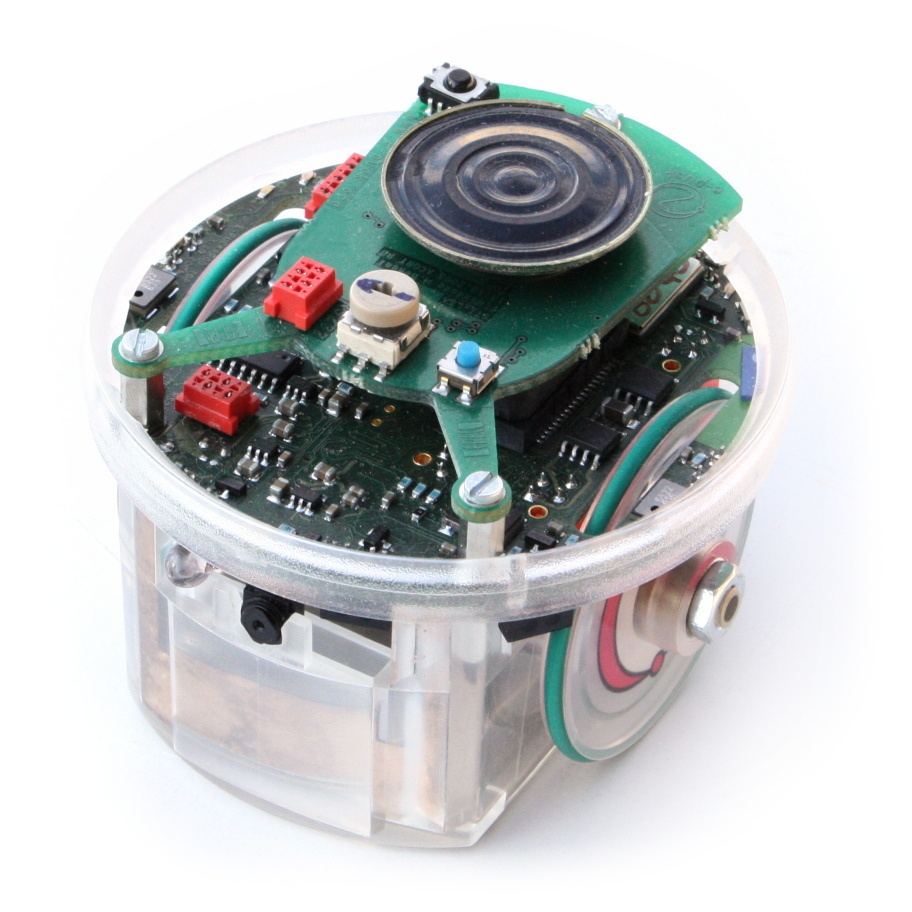
\includegraphics[width=0.7\textwidth]{./Figures/E-puck.jpg}
		\rule{35em}{0.5pt}
	\caption[swarm]{E-puck. Imagen extraida de Wikipedia}
	\label{fig:epuck}
\end{figure}


%-----------------------------------
%	SUBSECTION 4
%-----------------------------------

\subsection{3pi Robot}

Pololu, la misma marca que tiene desarrollo de varios tipos de motores para robótica y PCB para controlarlos, diseño el 3pi Robot. Es un robot bastante más económico que el e-puck, cuyo valor es 99.95USD ref. Sparkfun. También tiene dos ruedas para desplazarse de forma diferencial, 5 sensores de reflectancia, un LCD de 8x2 caracteres, un buzzer y tres botones para que el usuario pueda programarlos. Todos estos dispositivos están conectados a un microcontrolador ATmega328. Su velocidad es de 90 cm/s.

El 3pi fue diseñado especialmente como un robot seguidor de lineas y solucionador de laberintos. Existen varios videos que muestran la asombrosa velocidad de estos robots para solucionar un laberinto. Se programa en C, pero como posee un microcontrolador ATmega es posible hacer uso del bootloader Arduino y programarlo con ese IDE. Usa 4 baterias AAA y trae 4 LEDs.

Para el modelo que se planteó en este trabajo hace falta un módulo de comunicación inalámbrica, y el 3pi no tiene. Para usar esta alternativa es necesario sumarle a su precio 26USD, que es el precio del módulo XBee 1[w] serie 2 que se vende en Sparkfun.

\begin{figure}[htbp]
	\centering
		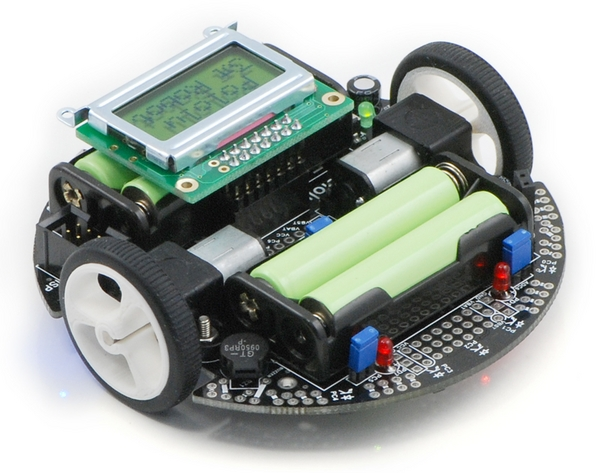
\includegraphics[width=0.7\textwidth]{./Figures/3pi.jpg}
		\rule{35em}{0.5pt} 
	\caption[swarm]{3pi Robot, simple y económico pero no tiene comunicación inalámbrica. Imagen extraida de http://www.skpang.co.uk}
	\label{fig:3pi}
\end{figure}

Una tabla comparativa resume las principales caracteristicas de los robot: Kilobot\footnote{http://www.k-team.com/mobile-robotics-products/kilobot/specifications}, E-puck\footnote{http://www.gctronic.com/doc/index.php/E-Puck} y 3pi\footnote{http://www.pololu.com/catalog/product/975/specs}.

\begin{table}\small
    \begin{tabular}{l|lll}
    ~                        &    Kilobot                    &    E-puck                                           &    3pi                          \\ \hline
       Procesador            &    ATmega   328 @ 8MHz &    dsPIC 30 CPU @ 30 MHz                &    ATMega328                    \\
       Memoria               &    32 KB   Flash              &    114 KB   Flash                                   &    32 KB   Flash                \\
       Autonomía             &    3 meses   (modo sleep)     &    3 horas                                          &    45   minutos                 \\
       Cargador              &    opcional                   &    opcional                                         &    opcional                     \\
       Comunicacion          &    Infrarojo(IR)              &    Bluetooth                                        &    opcional                     \\
       Sensores              &    Potencia   recibida IR     &    Proximidad,   camara, otros &    5   Reflectancia \\
       Movimiento            &    2 motores   vibración      &    2 motores   diferencial                          &    2 motores   diferencial      \\
       Output                &   1 (RGB) LED                 &    8 (RGB)   LED + parlante                         &    LCD 8x2 + buzzer             \\
       Diametro              &    33 [mm]                    &    70 [mm]                                          &    95[mm]                       \\
       Alto                  &    34[mm]                     &    50 [mm]                                          &    32[mm]                       \\
       Software &    Básico                     &    Complejo                                         &    Básico                       \\
       Programación          &    WinAVR                     &    MPLAB                                            &    Arduino                      \\
       Precio USD            &    1.161 (10 pack)            &    900                                              &    100                          \\
    \end{tabular}
    \label{table:comparacion}
    \caption {Comparación de robots Kilobot, e-puck y 3pi.}
\end{table}


%-----------------------------------
%	SECTION 3
%-----------------------------------

\section{Necesidades de mercado}
\begin{figure}[htbp]
	\centering
		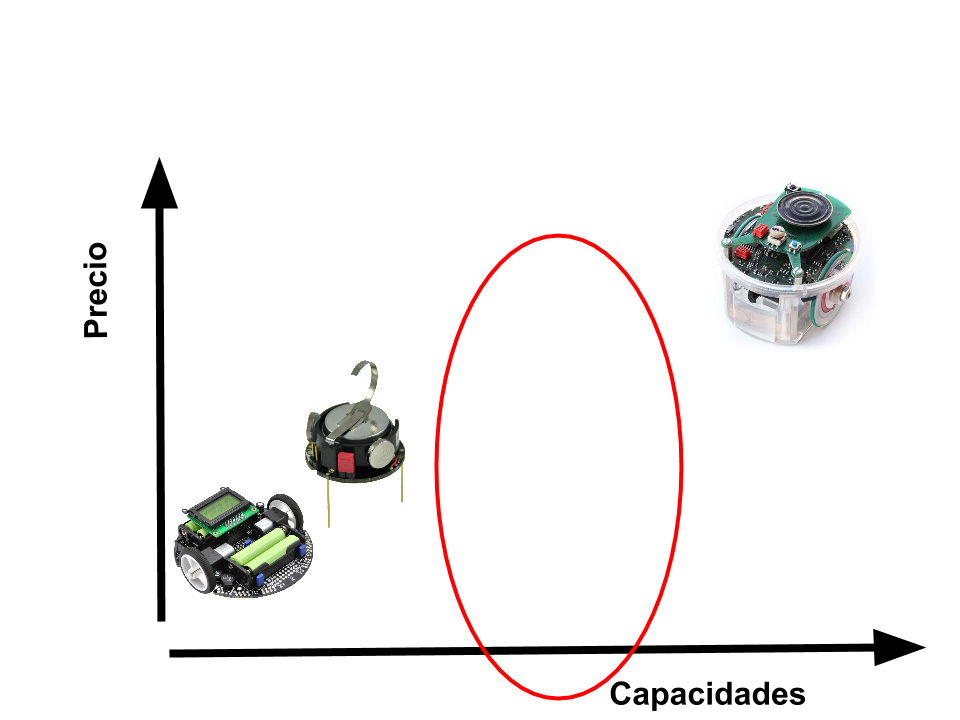
\includegraphics[width=0.8\textwidth]{./Figures/nicho.png}
		\rule{35em}{0.5pt}
	\caption[nicho]{Nicho de mercado}
	\label{fig:nicho}
\end{figure}

De los robots estudiados destaca en sus prestaciones el e-puck, pero este tiene dos grandes problemas para ser usado por gente que no es especialista en robots. Uno es que tiene demasiado hardware, lo que tiende a confundir y aumentar costos. Dos, que para su comunicación inalámbrica hace uso de Bluetooth, protocolo que no soporta las redes Mesh para hacer de manera simple el control de muchos dispositivos en una red. Hace falta un robot capaz de controlarse de forma inalámbrica, simple de construir y fácil de usar. Además debe ser económico para poder construir varios. Se pretende hacer uso de tecnologías como impresoras 3D y  de desarrollo como el Open Hardware.


%----------------------------------------------------------------------------------------
%	SUBSECTION 3
%----------------------------------------------------------------------------------------

\subsection{Usos Académico}

Un enjambre de robots puede presentar muchas ventajas dentro del aula. Si se tiene un sistema de fácil uso para los alumnos, el profesor puede asignar una tarea a un grupo de estudiantes donde cada uno tiene la responsabilidad de controlar o programar un robot para que el conjunto logre una meta determinada como ordenar unos bloques o hacerse cargo de regar un pequeño huerto. Abusando un poco del concepto de la colectividad, incluso pueden generarse tareas donde cada colegio se especializa en un tipo de tareas para luego juntar los distintos robots y probar cómo interactúan.

Tener un setup con robots que demuestren un comportamiento colectivo puede ser muy ventajoso para ayudar a niños con trastornos como el Asperger a practicar sus habilidades para reconocer estos mismo comportamientos.

\subsection{Usos Militar}

\subsection{Usos Doméstico}


% Chapter Template

\chapter{MODI} % Main chapter title

\label{Chapter3} % Change X to a consecutive number; for referencing this chapter elsewhere, use \ref{ChapterX}

\lhead{Capítulo 3. \emph{MODI}} % Change X to a consecutive number; this is for the header on each page - perhaps a shortened title

%----------------------------------------------------------------------------------------
%	SECTION 1
%----------------------------------------------------------------------------------------

\section{Diseño}

\begin{figure}[htbp]
	\centering
		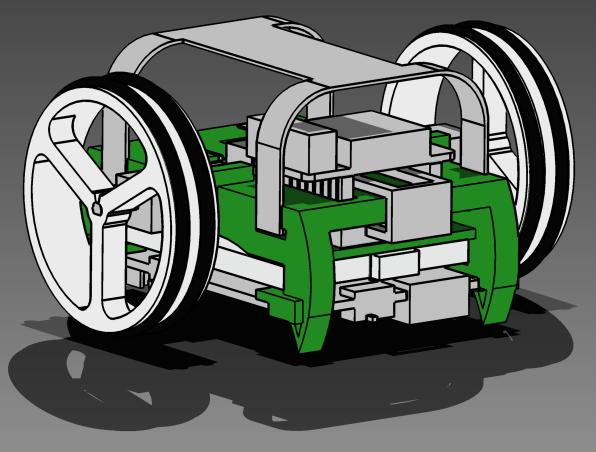
\includegraphics[width=0.8\textwidth]{./Figures/MODI/render.png}
		\rule{35em}{0.5pt}
	\caption[Robot MODI]{robot MODI (sigla para Modular Intelligence)}
	\label{fig:MODI}
\end{figure}

La función principal de MODI es ser una plataforma móvil de fácil acceso. Existe un repositorio en GitHub  \footnote{https://github.com/FabLabUChile/modi} donde se tienen los códigos actualizados para controlar y construir robots MODI. Una lista con componentes extras para comprar se encuentra en la Figura \ref{fig:BOM}.
\linebreak 

\textbf{Requerimientos de desarrollo}

\begin{itemize}
\item Simple de fabricar
\item Open Source
\item Fabricable en un Fab Lab
\item Componentes extras necesarios, de fácil acceso
\item Minimizar la cantidad de componentes mecánicos extras necesarios
\item Carga Autónoma con celda solar
\item Seguimiento de grupo
\item Control individual del color de cada MODI
\item Movimiento simple de cada robot de forma independiente
\end{itemize}

%-----------------------------------
%	SECTION 2
%-----------------------------------

\section{Construcción}

La Construcción de un robot implica el diseño en computador de varios componentes. Estos pueden ser circuitos electrónicos (PCB), software de control y piezas mecánicas. Uno de los requerimientos principales de desarrollo es que sea simple de fabricar, es por esto que en el resultado final se reflejan las horas de diseño.

%-----------------------------------
%	SUBSECTION 2
%-----------------------------------
\subsection{Fabricación Digital vs Análoga}
Cuando se quiere pasar una idea al mundo real es necesario un proceso de fabricación. Dependiendo de la cantidad de herramientas que se tenga es más o menos fácil la tarea. Desde el comienzo hasta hace un par de años, quienes se dedican a construir robots, debían construir de manera \textit{artesanal} donde es imposible que las piezas queden todas iguales y el tiempo empleado era bastante. Hoy en día existe una gran alternativa que surge como un nuevo paradigma, la Fabricación Digital. Las impresoras 3D, que no son más que un extrusor montado en un sistema con ejes que le dan 3 grados de libertad, permiten desde un modelo en un computador, obtener un objeto real hecho en plástico. También existe otro tipo de máquinas que permite hacer diseños en 2D, estas son las cortadoras LASER. La primera versión de MODI fue construido usando planchas de madera MDF y acrílico, cortados en LASER.

Utilizando una impresora 3D Makerbot Replicator 1 se hizo esta primera versión con piezas plásticas.

\begin{figure}[htbp]
	\centering
		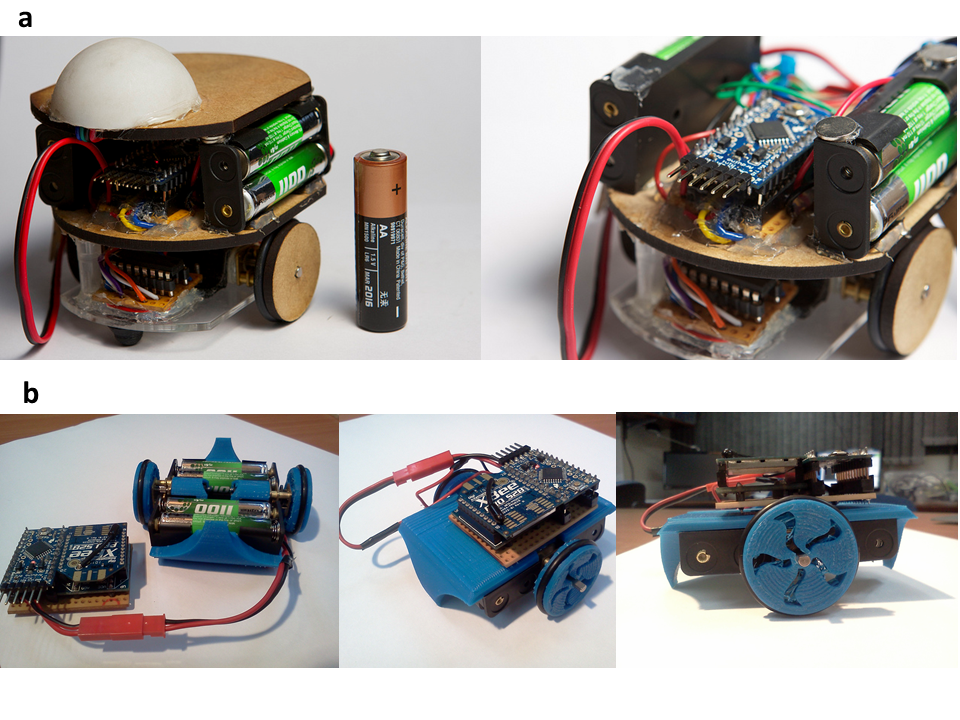
\includegraphics[width=0.8\textwidth]{./Pictures/modi_analogToDigital.png}
		\rule{35em}{0.5pt}
	\caption[modireplicator]{Primera versión de MODI usando técnica de \emph{ Fabricación Digital }con chasis de plástico construido con una MakerBot Replicator 1}
	\label{fig:modireplicator}
\end{figure}

Esta versión presentaba el problema de involucrar demasiadas partes que debían ser hechas por una persona. El microcontrolador, junto con la radio inalámbrica se colocaron en una placa electrónica para prototipado, más adelante se puede ver que fueron reemplazados por una PCB llamada Arduino FIO, que es una plataforma de desarrollo Arduino junto con un socket Xbee. Otro factor clave para descartar esta versión es que utiliza 4 pilas AAA que necesitan ser removidas para poder ser recargadas, lo que impide que en futuras versión exista la posibilidad de una carga autónoma por parte de los Robots. La versión actual de MODI permite su carga por medio de un puerto Mini USB, panel solar y de forma inalámbrica.

Aunque han bajado los precios de las maquinas para prototipado rápido, aún no están al alcance de todas las personas. Es por esto que existen los Fab Labs (acrónimo del inglés Fabrication Laboratory), que según Wikipedia es, \textit{"un espacio de producción de objetos físicos a escala personal o local que agrupa máquinas controladas por ordenadores. Su particularidad reside en su tamaño y en su fuerte vinculación con la sociedad."} Los Fab Labs están por todo el mundo, Figura \ref{fig:Fablabs}. MODI fue concebido como un proyecto del Fab Lab de la Universidad de Chile y por esto es posible reproducirlo en cualquier Fab Lab. En Chile, además del Fab Lab de la Universidad de Chile están: Design LAB UAI, Fab Lab Santiago y Stgo MakerSpace. 

\begin{figure}[htbp]
	\centering
		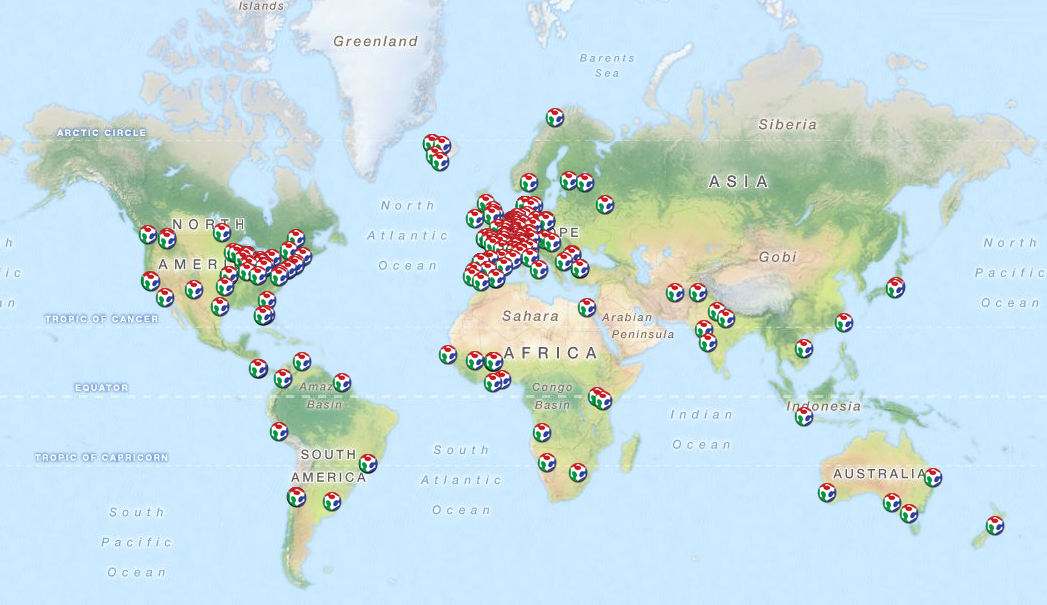
\includegraphics[width=0.8\textwidth]{./Figures/map.png}
		\rule{35em}{0.5pt}
	\caption[Fablabs]{Mapa actual de lugares en el mundo que cuentan con un Fab Lab. En Chile a la fecha existen 3. Imagen obtenida desde fablabamersfoort.nl/fablabs/}
	\label{fig:Fablabs}
\end{figure}	

%-----------------------------------
%	SUBSECTION 3
%-----------------------------------
\subsection{Software CAD}

CAD viene de sus siglas del Inglés, Computer-aided design, y se refiere a un diseño asistido por herramientas computacionales. Profesionales como ingenieros, arquitectos y del área del diseño por lo general son los que hacen más uso de estas herramientas.

Parte de la definición de Wikipedia es, \textit{”... se pueden dividir básicamente en programas de dibujo en dos dimensiones (2D) y modeladores en tres dimensiones (3D). Las herramientas de dibujo en 2D se basan en entidades geométricas vectoriales como puntos,líneas, arcos y polígonos, con las que se puede operar a través de una interfaz gráfica....”}

Durante el transcurso del proyecto se trabajó con varios softwares CAD. El primero fué SketchUp 8 de Google, que permite fácilmente hacer bocetos de lugares y cuenta con una importante biblioteca de modelos para incluir en el diseño. Rápidamente se pudo hacer un scketch utilizando modelos descargados de Internet , Figura~\ref{fig:setup}.

El diseño del chasis junto con las ruedas y demás partes plásticas, se hizo en un comienzo con SolidWorks 2012 y luego por ser más simple de usar, Inventor 2013 de Autodesk. Ambos softwares permiten generar modelos en 3D para luego exportar el diseño al formato STL que es estándar para prototipar en plástico.


\begin{figure}[htbp]
	\centering
		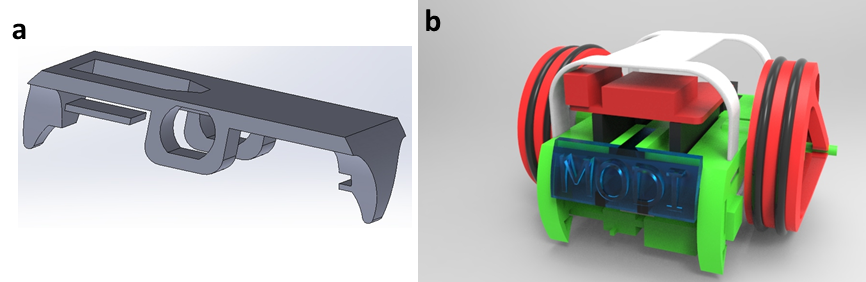
\includegraphics[width=0.9\textwidth]{./Figures/MODI/compRender.png}
		\rule{35em}{0.5pt}
	\caption[ModiSolidWorks]{Primer Chasis de MODI, realizado con SolidWorks 2012. Esta versión sirve solo como prueba de concepto ya que no tiene espacio para las conexiones eléctricas necesarias}
	\label{fig:MODISolidWork}
\end{figure}	

Luego de varias iteraciones se lográ este modelo, Figura \ref{fig:render3} que tiene cinco piezas. 



%-----------------------------------
%	SUBSECTION 4
%-----------------------------------
\subsection{Impresora 3D} \label{cap:impresora3D}

Parte importante de este trabajo se realizó con impresoras 3D. Estas existen desde los años 80' y hasta hace algunos años por su precio y tamaño eran de dificil acceso. Utilizan distintas tecnologías, las que se utilizaron en el proceso de este trabajo son las FDM, sigla del ingles "Fused deposition modeling" donde un cabezal extrusor de plástico se mueve en el plano xy depositando capa por capa de material mientras avanza en el eje z.

\begin{figure}[htbp]
	\centering
		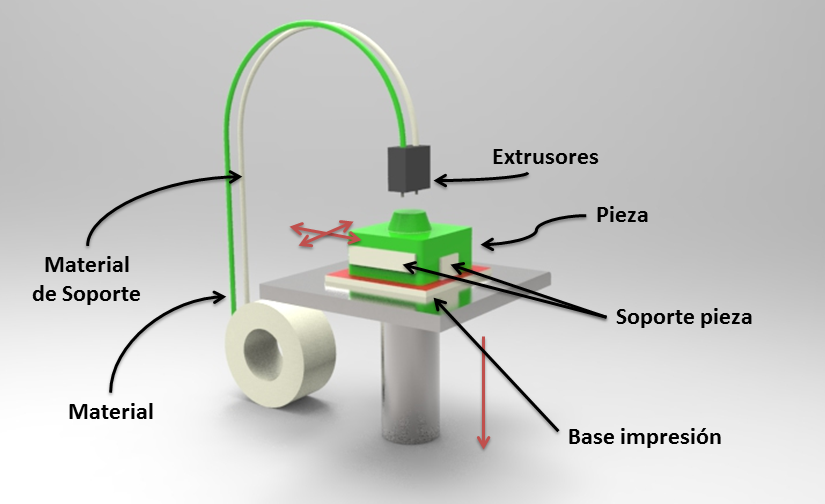
\includegraphics[width=\textwidth]{./Figures/3Dprint.png}
		\rule{35em}{0.5pt}
	\caption[3Dprint]{Modelo de funcionamiento para impresoras 3D MDF. Tiene dos materiales, uno para construir la pieza y otro que funciona como soporte estructural para la impresión, además existe una base que se calienta para sujetar la pieza mientras se construye.}
	\label{fig:3Dprint}
\end{figure}	

Primero se utilizó la 3D Touch Dual de la empresa Bit from Bytes, que permite hacer modelos de hasta 185 x 273 x 200[mm], con una buena resolución de 0.125[mm]\footnote{teambastech.com/Store/index.php?route=product/product\&product\_id=205} cada capa en eje z. Luego por facilidad de uso y menor tiempo de impresión se usa una impresora MakerBot Replicator 1

\begin{figure}[htbp]
	\centering
		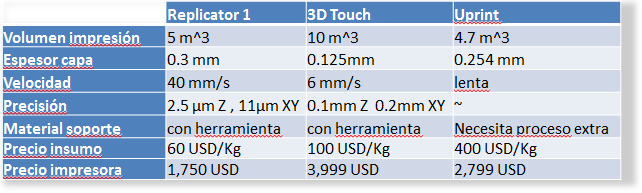
\includegraphics[width=\textwidth]{./Figures/tabla_impresoras.png}
		\rule{35em}{0.5pt}
	\caption[Replicator1]{Replicator 1 de Makerbot, impresora 3D FDM utilizada para prototipar chasis y ruedas de robot MODI. En Laboratorio de Síntesis de maquinas inteligentes de la Universidad de Chile, junto a la Fab@Home y 3DTouch.}
	\label{fig:replicator}
\end{figure}


\begin{figure}[htbp]
	\centering
		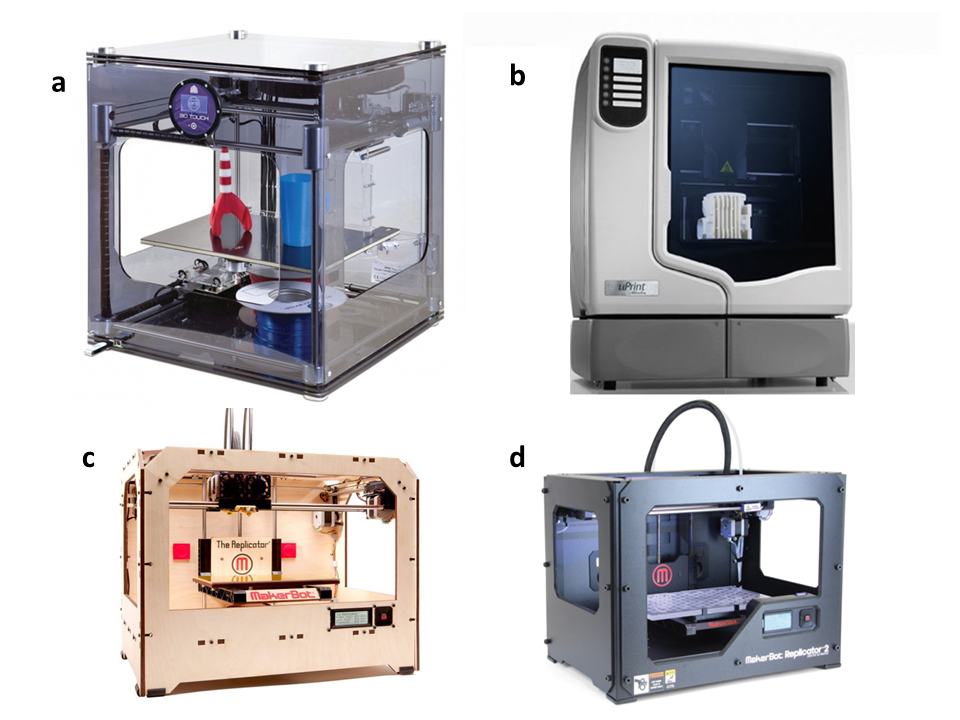
\includegraphics[width=\textwidth]{./Figures/impresoras.png}
		\rule{35em}{0.5pt}
	\caption[Replicator1]{Replicator 1 de Makerbot, impresora 3D FDM utilizada para prototipar chasis y ruedas de robot MODI. En Laboratorio de Síntesis de maquinas inteligentes de la Universidad de Chile, junto a la Fab@Home y 3DTouch.}
	\label{fig:replicator}
\end{figure}	
\FloatBarrier

%-----------------------------------
%	SUBSECTION 5
%-----------------------------------
\subsection{Diseño PCB}

En los primeros prototipos un problema que se repetía constantemente son las conexiones entre los sistemas que componen al robot. Son 15 conexiones que unen distintos componentes, Figura \ref{fig:Diagrama cables}. Por esto es necesario un PCB que permita reducir al mínimo el espacio necesario para para energizar y comunicar los elementos. El requerimiento principal es poder fabricarse con una fresa CNC como la Roland Modela MDX-20, por lo que es necesario diseñar un PCB de una sola capa. Se utilizó Eagle como software para el diseño del diagrama eléctrico y PCB, el resultado se puede ver en la Figura \ref{fig:pcbeagle}.


\begin{figure}[htbp]
	\centering
		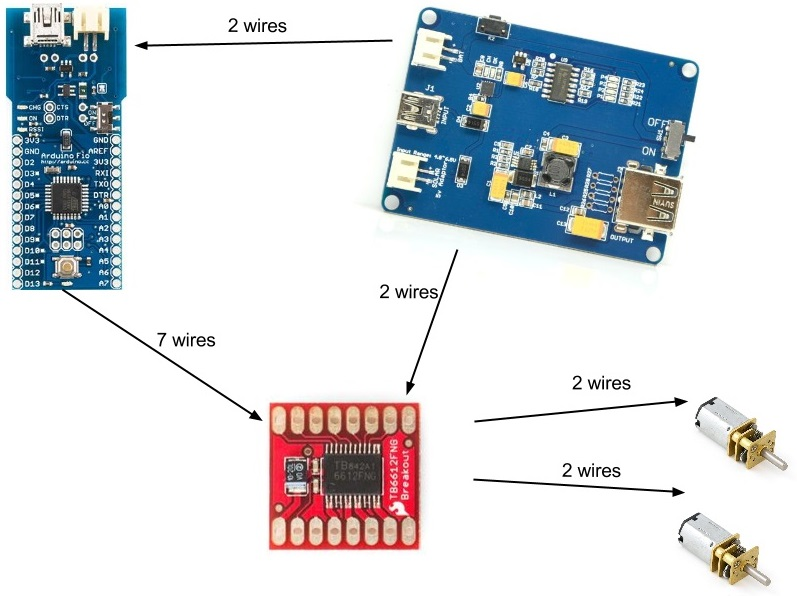
\includegraphics[width=0.6\textwidth]{./Figures/Diagrama.jpg}
		\rule{35em}{0.5pt}
	\caption[cables]{15 conexiones que unen distintos componente.}
	\label{fig:Diagrama cables}
\end{figure}	

\begin{figure}[htbp]
	\centering
		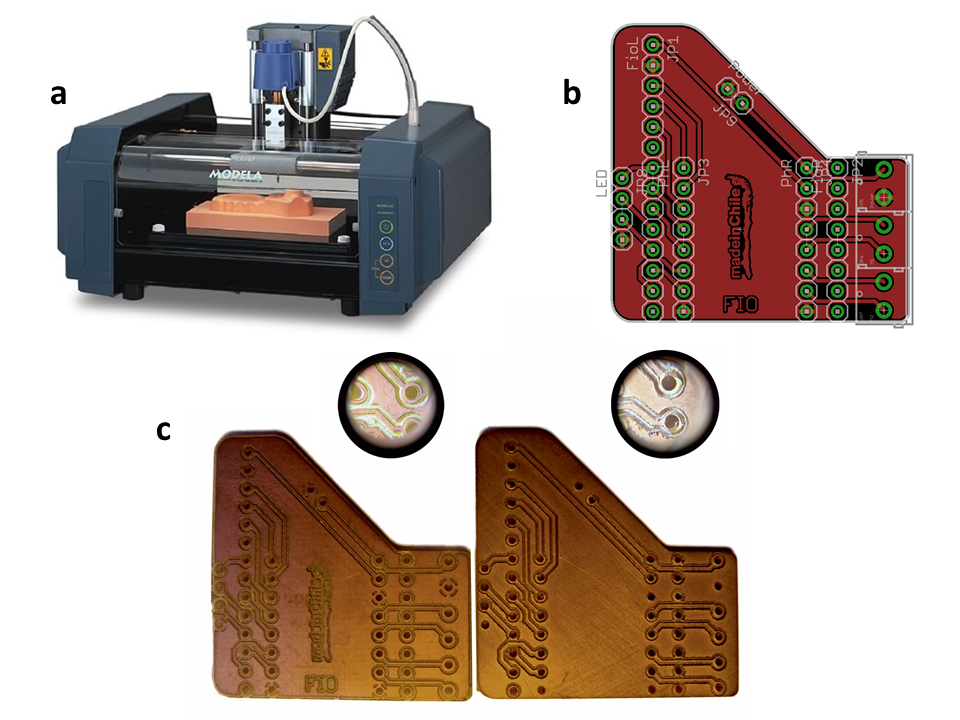
\includegraphics[width=0.9\textwidth]{./Figures/modi/pcb.png}
		\rule{35em}{0.5pt}
	\caption[MDX20]{Roland Modelo MDX-20 usada para hacer PCB y modelos 3D. Imagen tomada de roland.com, MODIBoard es una PCB diseñada para poder conectar de forma simple los diversos componentes electrónicos. Conecta: Arduino Fio, Lipo Rider Pro, Motor Driver, LED RGB y Motores, Misma PCB fresada en dos maquinas diferentes. Se puede apreciar en el detalle aumentado 60x, la importancia de contar con una buena resolución de fresado. En especial es necesario para tener un buen pad }
	\label{fig:MDX20}
\end{figure}

%-----------------------------------
%	SECTION 2
%-----------------------------------

\section{Componentes electrónicos}

\begin{figure}[htbp]
	\centering
		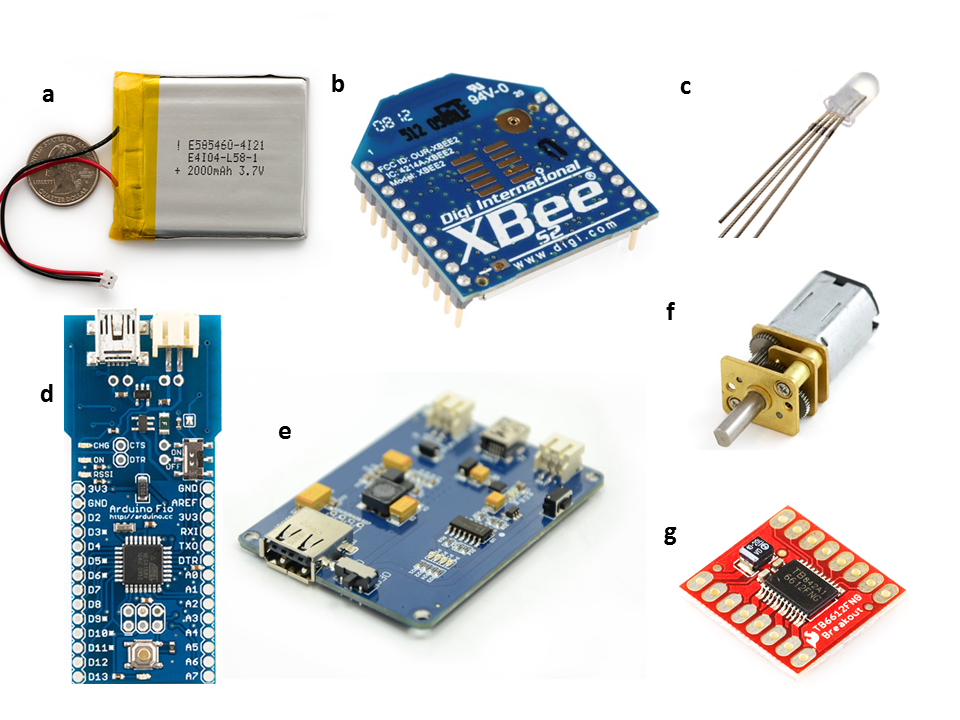
\includegraphics[width=\textwidth]{./Figures/MODI/compElo.png}
		\rule{35em}{0.5pt}
	\caption[Componentes Electrónicos]{\textbf{a.} Batería LIPO 2,000 mAh, \textbf{b.} XBee, \textbf{c.} LED Rgb difuso, de esta manera se obtiene un ángulo de visión mucho más amplio, \textbf{d.} Arduino Fio, \textbf{e.} Lipo Rider Pro,\textbf{ f.} Motor DC 30:1 \textbf{g.} Motor Driver 1A Dual TB6612FNG.}
	\label{fig:ledRGB}
\end{figure}

MODI está compuesto por varios componentes electrónicos que implementan tecnologías nuevas. De forma sencilla el usuario puede hacer uso de todas estas, que por ser Open Source tienen una amplia documentación. Su uso en colegios, talleres y universidades, por ser de bajo costo, y sin partes externas extremadamente frágiles, es una excelente herramienta para iniciar a alumnos en temas como la Programación, Robótica, Comunicación Inalámbrica y Visión Artificial, entre otros, sin los miedos asociados a utilizar un equipo costoso y delicado.

El robot MODI es pequeño y de fácil construcción con las herramientas de Fabricación Digital que se puede encontrar en un FabLab. Tiene un pequeño microcontrolador \textbf{Arduino} que controla dos motores, y un \textbf{XBee} para la comunicación inalámbrica con un computador central que usando cualquier lenguaje de programación con comunicación serial puede controlar uno o más robots. La posición de cada robot se obtiene con tags \textbf{Fiduciales}, que permiten por medio de una cámara cenital saber la coordenada y rotación de cada uno. En esta primera aplicación es necesario contar con autonomía energética por lo que se incluye una batería lipo de 2000[mAh] junto a un módulo que carga la batería y eleva el voltaje de salida a 5[v]. Este el módulo de carga, \textbf{Lipo Rider Pro}, tiene además la ventaja de permitir distintos tipos de carga, como una celda de carga solar o un sistema de carga inalámbrica por medio de bobinas. Tener la posibilidad de cargar una batería con luz solar o por medio de forma inalámbrica hace posible el hacer experimentos que necesiten estar funcionando semanas sin la intervención de un humano para cargar cada uno.

%-----------------------------------
%	SUBSECTION 1
%-----------------------------------
\subsection{Arduino FIO}
El Arduino FIO,\ref{fig:} ha sido diseñado por Shigeru Kobayashi, es una placa para microcontrolador basada en el ATmega328P. Funciona a 3.3V y 8 MHz. Tiene 14 pines de I/O digitales (de los cuales 6 pueden usarse como salidas PWM), 8 entradas analógicas, un oscilador en placa, un botón de reinicio (reset), y agujeros para montar conectores de pines. Tiene conexiones para una batería de polímero de Litio e incluye un circuito de carga a través de USB. En el reverso de la placa tiene disponible un zócalo para módulos XBee.

El Arduino FIO está diseñado para aplicaciones inalámbricas. El usuario puede subir sus sketches con un cable FTDI o una placa adicional adaptadora Sparkfun. Además, si utiliza un adaptador de USB a XBee modificado (como el USB Explorador de XBee), el usuario puede subir sketches de forma inalámbrica. La tarjeta viene sin conectores pre-montados, permitiendo el uso de diversos tipos de conectores o la soldadura directa de los cables. La tabla \ref{table:Especificaciones Fio} resume sus características principales.

%-----------------------------------
%	SUBSECTION 2
%-----------------------------------
\subsection{Motores DC}
Este motor Pololu es muy pequeño (largo: 9.27 mm), por lo mismo usa muy poca corriente y tiene una caja de reducción metálica de 30:1. El eje tiene forma de D.

Pese a no ser la alternativa más económica, estos motores han sido muy difundidos para su uso en robótica por su bajo consumo y alto torque. La tabla \ref{fig} resume sus características principales.

%-----------------------------------
%	SUBSECTION 3
%-----------------------------------
\subsection{XBee}

Los dispositivos con los cuales interactuamos a diario poseen acceso a distintos tipos de sistemas de comunicación. Los llamados “Smartphone” cuentan con diversas antenas para conectarse, WIFI, Bluetooth, red celular,  por nombrar algunas. Estamos en un momento en que las comunicaciones son una de las claves tecnológicas que nos permiten cumplir con tareas que para nuestros abuelos eran imposibles de hacer en un día. Es claro que un sistema con varios o cientos de robots también necesitan comunicarse. 

Para comunicar un robot con otro pueden usarse diversas técnicas. Dependiendo del área en particular que sea del interés del científico, los robot pueden comunicarse por medio de sensores de proximidad o tacto, para saber que hay otro cerca, pueden tener un sistema de visión artificial con una cámara a bordo que le permita “ver” el entorno al robot, con parlantes y micrófonos pueden emitir algún ruido que sea interpretado por su entorno, o lo mismo con sensores de otros tipos.

El robot que se construyó para hacer las pruebas cuenta con un sistema externo de visión artificial que permite obtener posición y orientación de cada robot. Esta información es transmitida a cada robot por medio del protocolo zigbee implementado en los chip XBee de la empresa Digi, Figura \ref{fig:xbee}. Esto permite comunicar un alto número de robots, con muy poco consumo energético y de manera relativamente simple. Se escogió usar visión artificial sobre el sistema para bajar los costos individuales de los robots y XBee por ser el estándar en la industria en redes de sensores inalámbricos. Cabe destacar que los robots que existen en el mercado no incluyen XBee, y los que lo traen lo hacen como accesorio. 

%-----------------------------------
%	SUBSECTION 3
%-----------------------------------
\subsection{Lipo Rider Pro}

El LiPo Rider Pro es una versión mejorada del LiPo Rider, que es una fuente de poder para alimentar distintos gadget con energía verde. Esta placa permite alimentar con 5V distintos dispositivos. Puede obtener energía del sol o por medio de inducción magnética. También puede cargar un SmartPhone.

La Lipo Rider carga una batería de Litio Polímero. Posee una alta densidad de carga, 2000mAh a 3.7V. Figura \ref{fig:bateria}

%-----------------------------------
%	SUBSECTION 4
%-----------------------------------
\subsection{Motor Driver 1A Dual TB6612FNG}
El TB6612FNG motor driver puede controlar hasta dos motores DC, a una corriente constante de 1.2A (3.2A peak). Dos señales de entrada (IN1 y IN2) puede ser usadas para controlar el motor en una de cuatro modos de funcionamiento - CW, CCW, short-brake, y stop. Cada una de las salidas hacia los motores (A y B) se puede controlar separadamente, la velocidad de cada motor es controlada vía PWM con una frecuencia de hasta 100khz. El pin STBY debe colocarse en High para que el motor salga del estado Standby. Figura \ref{TB6612FNG}

\begin{figure}[htbp]
	\centering
		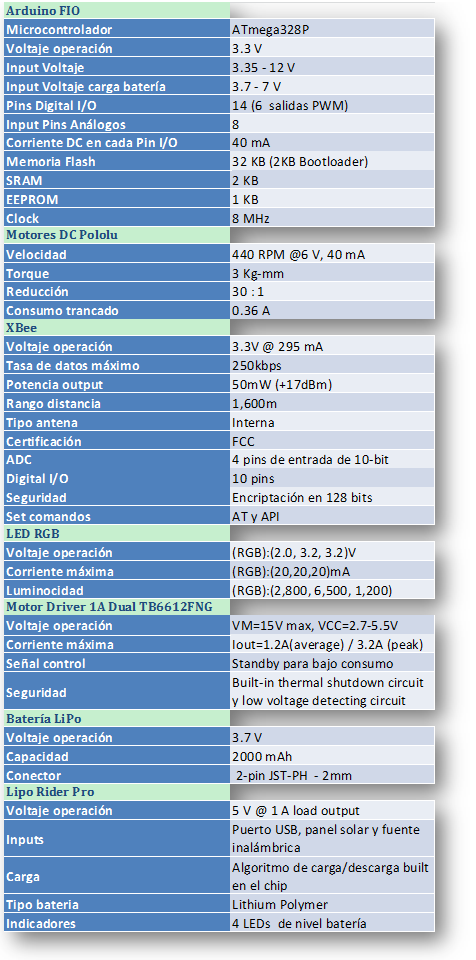
\includegraphics[width=0.8\textwidth]{./Figures/MODI/comparacionElo.png}
		\rule{35em}{0.5pt}
	\caption[Tabla ELO]{Resumen de las características más importantes de los componentes electrónicos que tiene MODI.}
	\label{fig:TablaElo}
\end{figure}


%-----------------------------------
%	SECTION 3
%-----------------------------------
\section{Componentes mecánicos}

Como se comentó en la sección \ref{cap:impresora3D}, las piezas del robot fueron diseñadas para ser construidas por una maquina de prototipado rápido del tipo FDM y se tener en cuenta la tolerancia mecánica de las piezas. En especial hay dos piezas: la rueda y el chasis, que se unen al motor. Esta unión debe quedar con un ajuste mecánico Forzado Medio \footnote{http://campuscurico.utalca.cl/\~ fespinos/Ajustes\%20y\%20tolerancias\%20mecanicas.pdf}, para que estas uniones queden fijas y las ruedas esten en el eje correspondiente.

El \textbf{Chasis} debe cumplir con la tarea de contener toda la electrónica y motores, las \textbf{Ruedas} permiten el desplazamiento y poseen dos canales para poner o-ring y así aumentar el roce con la superficie, el \textbf{Accesorio} tiene un sistema de anclaje al chasis que permite tener distintas carcasa y sensores, y el \textbf{Logo} sujeta parte de la electrónica contenida en el Chasis. 

La pieza que mas demora en construirse es el Chasis, que son 108 minutos en una Replicator 1 de MakerBot.

\begin{figure}[htbp]
	\centering
		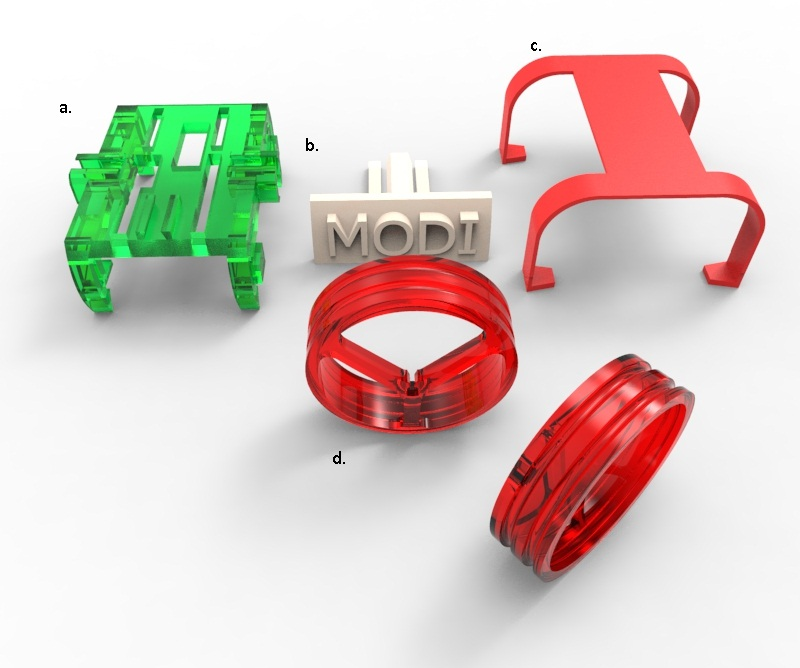
\includegraphics[width=\textwidth]{./Figures/MODI/piezas.jpg}
		\rule{35em}{0.5pt}
	\caption[Piezas 3D]{imágenes de todas las piezas renderizadas diseñadas.}
	\label{fig:Render Piezas 3D}
\end{figure}


%-----------------------------------
%	SECTION 4
%-----------------------------------

\section{Locomoción}
Existen distintas áreas donde se utilizan robots, dependiendo de la tarea a realizar es la movilidad que este debe tener. Algunos tienen complejos sistemas como la plataforma del proyecto Atlas (The Agile Anthropomorphic Robot) de Boston Dynamics, Figura \ref{fig:Atlas}. En nuestro caso, solo es necesario desplazarse sobre un superficie plana y por esto, en vez de tener costosos actuadores neumáticos, la solución más simple es contar con dos motores para poder tener un movimiento diferencial. Si se desea tener más información sobre los tipos de locomoción en robots con ruedas, ver esta pagina web\footnote{en.wikibooks.org/wiki/Robotics/Types\_of\_Robots/Wheeled}.


\begin{figure}[htbp]
	\centering
		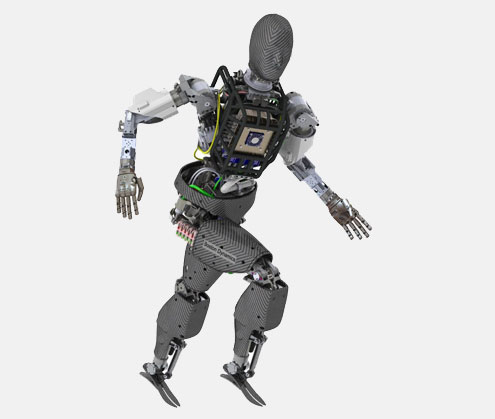
\includegraphics[width=\textwidth]{./Figures/AtlasCADlr.jpg}
		\rule{35em}{0.5pt}
	\caption[Atlas]{Atlas es un humanoide con gran movilidad, diseñado para poder usar herramientas humanas. Posee 28 grados de libertad con actuadores hidráulicos y la energía se le entrega por medio de un cable flexible. Imagen extraída de bostondynamics.com }
	\label{fig:Atlas}
\end{figure}


Para moverse MODI tiene dos motores DC \ref{fig:MotorDC}. Estos tienen una caja de reducción 30:1 que permiten aumentar el torque y disminuir la velocidad. La Figura \ref{fig:DCMotor} muestra la característica de estos. 

\begin{figure}[htbp]
	\centering
		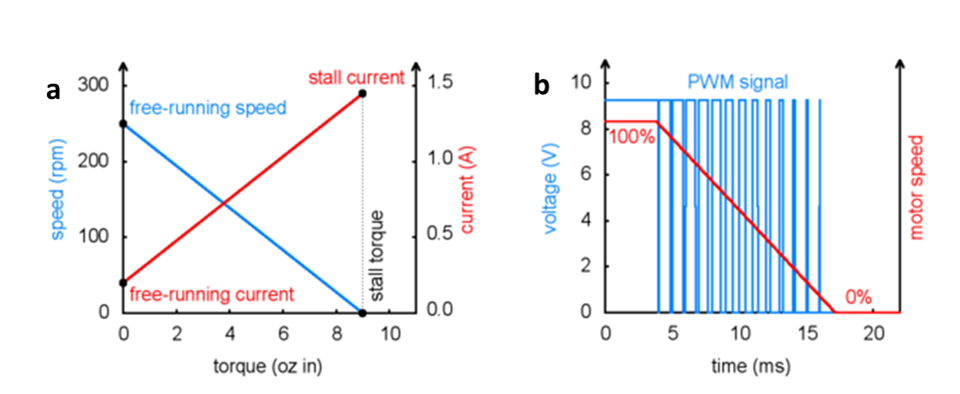
\includegraphics[width=\textwidth]{./Figures/graficosMotores.png}
		\rule{35em}{0.5pt}
	\caption[Gráficos Motor DC]{a. Operación motores: Corriente, velocidad y torque. Imagen extraída de pololu.com, b. Control de velocidad PWM, se observa como disminuye la velocidad según el ancho del pulso pwm.}
	\label{fig:DCMotor}
\end{figure}

El control de velocidad de los motores se hace con PWM, que es una señal periódica a la cual se le modifica el ciclo de trabajo. El sentido de giro es controlado con el chip TB6612FNG \ref{fig:DCMotor}(a.). Los valores van desde -255 a 255. Para más información sobre PWM y este chip ver esta pagina web \footnote{http://www.pololu.com/docs/0J21/5.c}. Este control además puede tener retro alimentación, se recomienda ver este video tutorial \footnote{http://www.youtube.com/watch?v=aE7RQNhwnPQ}.

\begin{figure}[htbp]
	\centering
		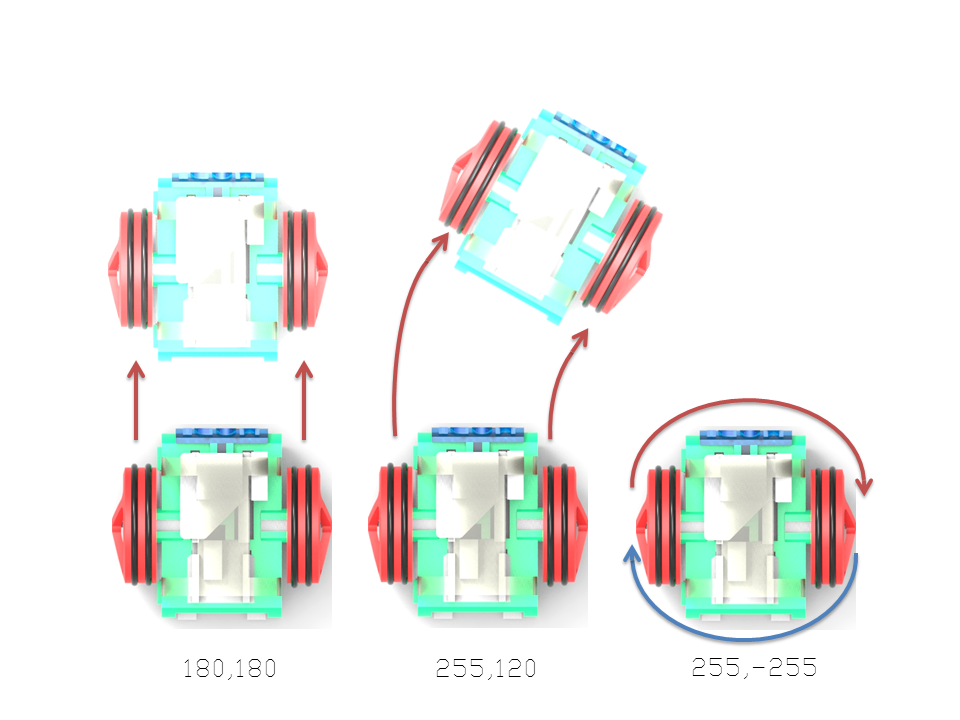
\includegraphics[width=0.8\textwidth]{./Figures/MODI/pwm.png}
		\rule{35em}{0.5pt}
	\caption[pwm]{Movimiento diferencial. A diferencia de un auto, MODI tiene dos motores que giran de forma independiente. Las distintas velocidades y sentido de giro determinan el angulo para girar. Si se necesita solamente rotar los motores deben girar en sentidos opuestos.}
	\label{fig:pwm}
\end{figure}

%-----------------------------------
%	SECTION 5
%-----------------------------------
\section{Implementación}

%-----------------------------------
%	SECTION 6
%-----------------------------------

\subsection{Setup}

Se desea realizar una investigación sobre el comportamiento colectivo de un grupo de robots, en el mundo real sin hacer uso de simuladores. Por esto  es necesario contar con un lugar físico donde poder activar los robot. Además para simplificar cada uno de los robots, estos no tienen sensores internos por lo que hay una cámara montada sobre el plano de movimiento de estos, para hacer Seguimiento Visual.
\begin{figure}[htbp]
	\centering
		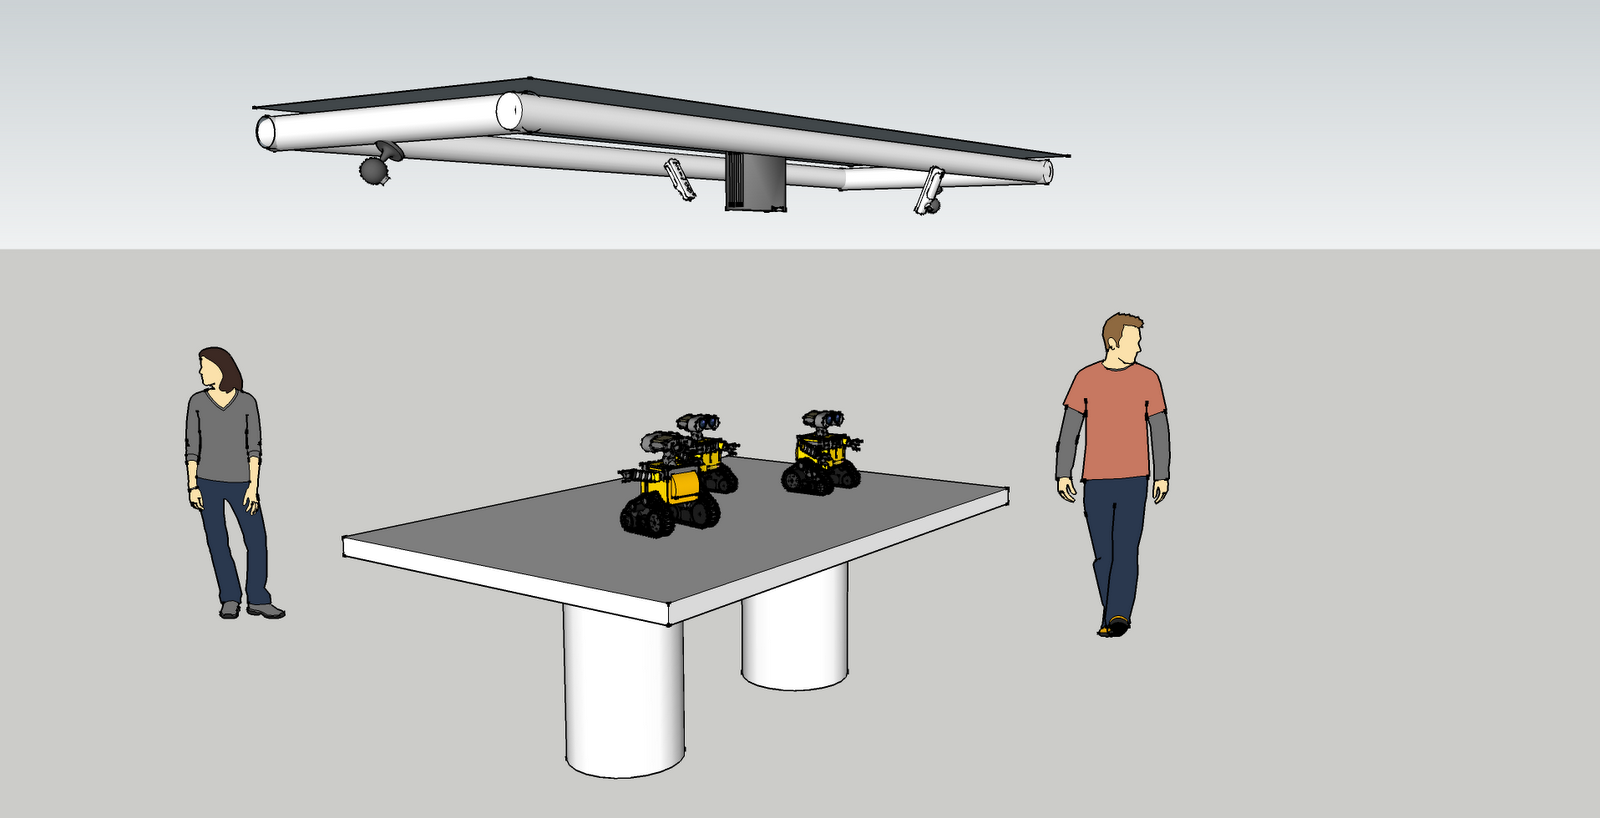
\includegraphics[width=\textwidth]{./Figures/setup.png}
		\rule{35em}{0.5pt}
	\caption[Setup Enjambre MODI]{Setup a montarse para hacer estudios de grupos de robots.}
	\label{fig:setup}
\end{figure}
\FloatBarrier
%-----------------------------------
%	SUBSECTION 6
%-----------------------------------

\subsection{Software}
Software, el cerebro del robot
Gracias a un puerto serial escuchando las instrucciones para mover los motores del robot, es bastante sencillo controlar a MODI desde el computador usando cualquier lenguaje que tenga una biblioteca para uso de puertos seriales.

A continuación algunos ejemplos de como controlar a MODI. El puerto serie en MODI tiene configurada una velocidad de 115200 y esta esperando los caracteres ‘w’,’a’,’d’ y ‘s’, como Adelante, Izquierda, Derecha y Atrás respectivamente. El código de MODI, el Firmware, se encuentra en el Git de MODI en Github.


\subsection{Tracking 2D}
Al igual que los seres vivos un robot necesita \textit{sentidos} o algún sistema sensorial para poder interactuar con su entorno. Estos pueden ser sensores IR para detectar objetos cercanos, cámaras o LASER para hacer un mapa del entorno o simplemente un pulsador que sea presionado cada vez que el robot colisiona. Para bajar costos, MODI actualmente no cuenta con sensores “onBoard”. Cada robot es comandado por un sistema que le dice donde donde está él, dónde están los demás y los límites del área de trabajo. Se diseñó de esta manera para simplificar la programación de cada robot.

reacTIVision es un framework open source, cross-platform, para realizar tracking rápido y robusto de tags fiduciales pegadas a objetos físicos. Ha sido diseñado como un toolkit para el desarrollo rápido multi-touch interactive surfaces. Este Framework fue desarrollado por Martin Kaltenbrunner y Ross Bencina en el Music Technology Group de la universidad de Pompeu Fabra en Barcelona, España. reacTIVision fue diseñado como sensor principal de la Reactable, un sintetizador modular tangible que ha marcado los standards en lo que a aplicaciones multitouch se refiere. Esta alternativa debe ir acompañada de otros elementos, como la cámara y el computador en el cual se ejecuta el software. 


\begin{figure}[htbp]
	\centering
		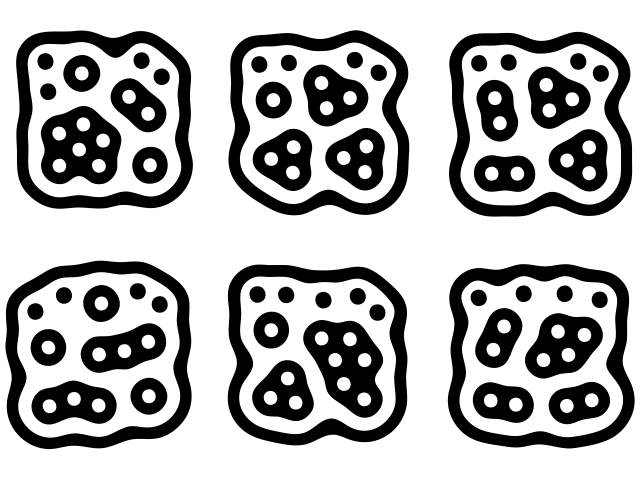
\includegraphics[width=0.8\textwidth]{./Figures/MODI/fiducial.png}
		\rule{35em}{0.5pt}
	\caption[Fiduciales usados como tag en reacTIVision]{Códigos fiduciales utilizados en reacTIVision. Estos códigos aunque parecen algo extraños para los seres humanos están diseñados de tal forma que es muy fácil diferenciar unos de otros y además obtener su orientación y posición en un software de análisis de imágenes. Se tiene un total de 216 configuraciones posibles de códigos.}
	\label{fig:Fiducial}
\end{figure}



%-----------------------------------
%	SECTION 7
%-----------------------------------

\subsection{Bill Of Material}

Con un precio total de ~180 USD, figura \ref{fig:BOM}, MODI se propone como una alternativa económica para construir un robot. Pensando en comprar desde Chile, son tres las tiendas en que se cotizaron los componentes. Es posible comprar todo desde internet. Para más detalles sobre la Lista de materiales ver \footnote{http://kitbom.com/otrab/modi} 
\begin{figure}[htbp]
	\centering
		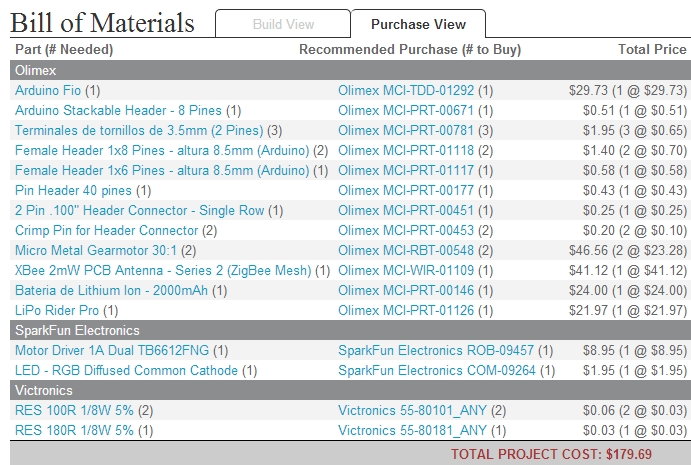
\includegraphics[width=\textwidth]{./Figures/MODI/kitbom.png}
		\rule{35em}{0.5pt}
	\caption[Bill Of Materials]{http://kitbom.com/otrab/modi}
	\label{fig:BOM}
\end{figure}

% Chapter Template

\chapter{Aplicaciones} % Main chapter title

\label{ChapterX} % Change X to a consecutive number; for referencing this chapter elsewhere, use \ref{ChapterX}

\lhead{Capitulo 4. \emph{Aplicaciones}} % Change X to a consecutive number; this is for the header on each page - perhaps a shortened title

%----------------------------------------------------------------------------------------
%	SECTION 1
%----------------------------------------------------------------------------------------

\section{Auto modelamiento}

Juan Cristobal Zagal y Hod Lipson \cite{ZagalL09} exploraron el comportamiento de un robot capaz de entrar en un proceso de self-reflection. Ellos estudiaron a un robot al cual se le programaron dos controladores, uno primitivo (primitive controller) y uno reflexivo (reflective controller) que puede observar al primero.

\begin{figure}[htbp]
	\centering
		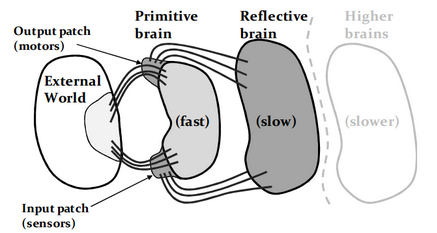
\includegraphics[width=0.7\textwidth]{./Figures/arquitectura_cerebro.png}
		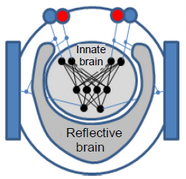
\includegraphics[width=0.4\textwidth]{./Figures/automodelado_epuck.png}
		\rule{35em}{0.5pt}
	\caption[Automodelado]{\textbf{Arriba:} Arquitectura de cerebros anidados usado en el trabajo de J.Zagal y H.Lipson, basado en modelos de M. Minsky. \textbf{Abajo:} Modelo de cerebros implementado en robot e-puck. Ambas imágenes  pertenecen a Juan Cristóbal Zagal.}
	\label{fig:Automodelado}
\end{figure}

El controlador reflexivo es capaz de determinar el control primitivo sin tener acceso directo  a sus estados internos si no que haciendo uso de ingeniería inversa al leer los input/output de éste. Acá se implementa como comportamiento que el robot (e-puck) debe alejarse de luces rojas y acercarse a azules. Se logra con una exploración mínima posible de hardware.

\begin{figure}[htbp]
	\centering
		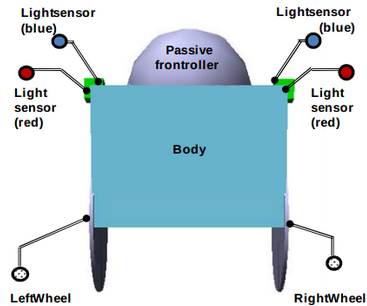
\includegraphics[width=0.4\textwidth]{./Figures/robotTest.png}
		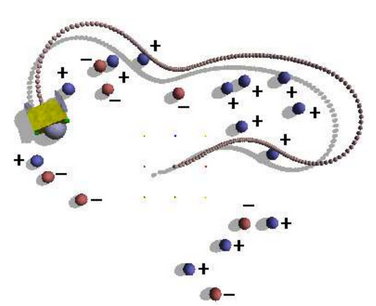
\includegraphics[width=0.5\textwidth]{./Figures/implementacion.png}
		\rule{35em}{0.5pt}
	\caption[Automodelado]{\textbf{Izquierda:} Arquitectura de cerebros anidados usado en el trabajo de J.Zagal y H.Lipson, basado en modelos de M. Minsky. \textbf{Derecha:} Modelo de cerebros implementado en robot e-puck. Ambas imágenes  pertenecen a Juan Cristóbal Zagal.}
	\label{fig:AutomodeladoTest}
\end{figure}


El diagrama del algoritmo que controla todo el proceso que se implementa como comportamiento para recuperarse de fallas puede verse en el anexo.

J. Bongard., V. Zykov y H. Lipson., logran que un robot se recupere de una falla inesperada de forma autónoma. Dicen que el robot puede recuperarse de manera autónoma haciendo uso de su (propio al robot) Self-modeling. Concretamente implementan sus algoritmos en un robot de 4 patas que utiliza una relación entre sus sensores y motores para indirectamente inferir su propia estructura.


Si se remueve una extremidad, el robot es capaz de generar una nueva forma de caminata que le permita cumplir con su misión que es avanzar.
En la figura \ref{fig:AutomodeladoLIPSON}, se describe un esquema del algoritmo. El robot realiza una acción física (A), al azar, luego se ejecuta la mejor acción que se encuentre en (C). A continuación genera varios auto-modelos que coincidan con las lecturas de los sensores obtenidas en (B). Aún no sabe cual es el modelo, por lo que en (C) genera varias acciones posibles que acotan la búsqueda de modelos.Después de varios ciclos de (A) a (C),  el modelo obtenido se utiliza en (E) para generar la secuencia de locomoción. La mejor secuencia de locomoción es probada físicamente en el robot. Se refina el modelo volviendo al paso (B) y en (D) pueden crearse nuevos comportamientos.

\begin{figure}[htbp]
	\centering
		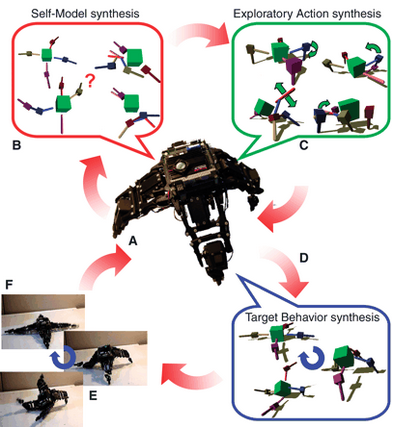
\includegraphics[width=0.5\textwidth]{./Figures/algoritmo_automodelo.png}
		\rule{35em}{0.5pt}
	\caption[AutomodeladoLIPSON]{Esquema del algoritmo que puede usar un robot para desplazarse haciendo uso de Automodelos. Imagen obtenida desde http://creativemachines.cornell.edu}
	\label{fig:AutomodeladoLIPSON}
\end{figure}


\section{Educacion}

%-----------------------------------
%	SUBSECTION 2.1
%-----------------------------------

\subsection{Subsection 2}

%----------------------------------------------------------------------------------------
%	SUBSECTION 3
%----------------------------------------------------------------------------------------
\subsection{Usos Académico}

Un enjambre de robots puede presentar muchas ventajas dentro del aula. Si se tiene un sistema de fácil uso para los alumnos, el profesor puede asignar una tarea a un grupo de estudiantes donde cada uno tiene la responsabilidad de controlar o programar un robot para que el conjunto logre una meta determinada como ordenar unos bloques o hacerse cargo de regar un pequeño huerto. Abusando un poco del concepto de la colectividad, incluso pueden generarse tareas donde cada colegio se especializa en un tipo de tareas para luego juntar los distintos robots y probar cómo interactúan.

Tener un setup con robots que demuestren un comportamiento colectivo puede ser muy ventajoso para ayudar a niños con trastornos como el Asperger a practicar sus habilidades para reconocer estos mismo comportamientos.

\subsection{Usos Militar}

\subsection{Usos Doméstico}
 
% Chapter Template

\chapter{Aplicaciones} % Main chapter title

\label{ChapterX} % Change X to a consecutive number; for referencing this chapter elsewhere, use \ref{ChapterX}

\lhead{Capitulo 4. \emph{Aplicaciones}} % Change X to a consecutive number; this is for the header on each page - perhaps a shortened title

%----------------------------------------------------------------------------------------
%	SECTION 1
%----------------------------------------------------------------------------------------
MODI en esencia es un Arduino con ruedas y control inalámbrico. Esto significa que para programarlo y hacer uso de él en un proyecto la curva de aprendizaje es rápida. Existen un sin fin de tutoriales donde se puede aprender lo básico para programar un Arduino y en un día ya se puede controlar de forma simple el movimiento del robot. Es por esto que MODI es indicado para usarse por cualquier persona que desee experimentar con robots y no tenga los conocimientos técnicos para construir uno desde cero. En las secciones siguientes se describen algunas aplicaciones posibles.

\section{Auto modelamiento}

Uno de los fines de MODI es poder ser utilizado para investigar el Auto modelamiento en robots, que permite a un robot sintetizar un comportamiento en base a la exploración de los posibles modelos de el mismo. La importancia de esta área radica en que actualmente los robots más difundidos hacen uso de un software llamado controlador, que por ejemplo para mover un robot del punto a al punto b controla las señales de cada moto, en base a como se encuentran ubicados en el espacio los motores, pero si un motor falla o si el robot en vez de tener ruedas tiene patas, no logra adaptarse. Juan Cristobal Zagal junto a Hod Lipson \cite{ZagalL09} exploraron el comportamiento de un robot capaz de entrar en un proceso autoreflexivo. Ellos estudiaron a un robot al cual se le programaron dos controladores, uno primitivo (primitive controller) y uno reflexivo (reflective controller) que puede observar al primero.

El controlador reflexivo es capaz de determinar el control primitivo sin tener acceso directo a sus estados internos, haciendo uso de ingeniería inversa al leer los input/output de éste. Acá se implementa como comportamiento que el robot (e-puck) debe alejarse de luces rojas y acercarse a azules. Se logra con una exploración mínima posible de hardware.

El diagrama del algoritmo que controla todo el proceso que se implementa como comportamiento para recuperarse de fallas puede verse en el anexo.

J. Bongard., et al. \cite{Bongard17112006}, logran que un robot se recupere de una falla inesperada de forma autónoma. Dicen que el robot puede recuperarse de manera autónoma haciendo uso de su (propio al robot) Self-modeling. Concretamente implementan sus algoritmos en un robot de 4 patas que utiliza una relación entre sus sensores y motores para indirectamente inferir su propia estructura.


Si se remueve una extremidad, el robot es capaz de generar una nueva forma de caminata que le permita cumplir con su misión que es avanzar.
En la figura \ref{fig:AutomodeladoLIPSON}, se describe un esquema del algoritmo. El robot realiza una acción física (A), al azar, luego se ejecuta la mejor acción que se encuentre en (C). A continuación genera varios auto-modelos que coincidan con las lecturas de los sensores obtenidas en (B). Aún no sabe cual es el modelo, por lo que en (C) genera varias acciones posibles que acotan la búsqueda de modelos.Después de varios ciclos de (A) a (C),  el modelo obtenido se utiliza en (E) para generar la secuencia de locomoción. La mejor secuencia de locomoción es probada físicamente en el robot. Se refina el modelo volviendo al paso (B) y en (D) pueden crearse nuevos comportamientos.

Utilizando el robot MODI es posible implementar el concepto de Self-modeling a un grupo de robots, donde el enjambre es capaz de adaptarse a distinta situaciones automodelando su forma grupal para por ejemplo lograr cruzar un puente 

\begin{figure}[htbp]
	\centering
		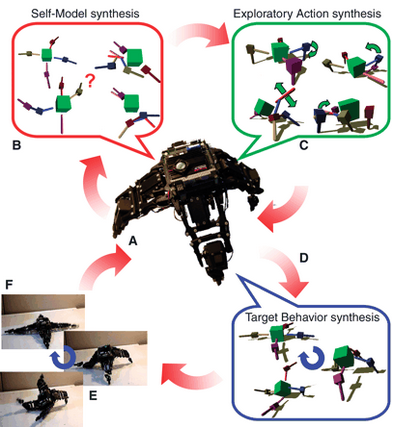
\includegraphics[width=0.7\textwidth]{./Figures/algoritmo_automodelo.png}
		\rule{35em}{0.5pt}
	\caption[Esquema algoritmo automodelado Hod Lipson]{Esquema del algoritmo que puede usar un robot para desplazarse haciendo uso de Automodelos. Imagen tomada de \cite{Bongard17112006}}
	\label{fig:AutomodeladoLIPSON}
\end{figure}


\section{Educación}

Un enjambre de robots puede presentar muchas ventajas dentro del aula. Si se tiene un sistema de fácil uso para los alumnos, el profesor puede asignar una tarea a un grupo de estudiantes donde cada uno tiene la responsabilidad de controlar o programar un robot para que el conjunto logre una meta determinada como ordenar unos bloques o hacerse cargo de regar un pequeño huerto. Abusando un poco del concepto de la colectividad, incluso pueden generarse tareas donde cada colegio se especializa en un tipo de tareas para luego juntar los distintos robots y probar cómo interactúan.

Tener un setup con robots que demuestren un comportamiento colectivo puede ser muy ventajoso para promover el aprendizaje de roles sociales si la docente a cargo programa los robot para que tengan distintos roles como Lider y participante. Este mismo juego de roles puede ayudar a los niños a generar estrategias y herramientas para enfrentarse al mundo. En síntesis haciendo juegos para los niños con los robots se puede tener su atención para reforzar su educación y favorecer en el desarrollo de habilidades y competencias. 

\section{Usos Militar}

Con un enjambre de robots, se puede simular una situación de catástrofe, donde es necesario poder desplegar un grupo de robots para hacer una tarea de reconocimiento y así poder buscar personas heridas o atrapadas.

%Imaginemos una situación hipotética donde un edificio es destruido, la búsqueda de sobrevivientes no es una tarea fácil, implica que rescatistas ingresen al lugar corriendo grave peligro, usualmente buscando a las víctimas en condiciones de poca visibilidad. Esto mismo podría ser ejecutado por un enjambre robótico que esté programado para buscar gente y que de manera colectiva recorra un área mucho mayor que 2 o 3 personas. Incluso un robot del mismo enjambre puede fallar, pero al ser un sistema distribuido el enjambre continúa funcionando, es un sistema muy robusto.

\section{Usos Doméstico}

Existen las aspiradoras Roomba, que sin necesidad de un operario humano pueden aspirar nuestras casas. Ellas recorren nuestro hogar y gracias a sus sensores pueden auto generar un mapa del entorno. Este modelo del hogar puede hacerse mucho más rápido si en vez de tener un solo robot, se tienen 20. El mismo concepto se puede aplicar en seguridad del hogar, donde se pueden tener varios mini robots haciendo rondas en el perímetro de nuestra casa y en forma colectiva abarcan lo más posible. Todas estas situaciones se pueden simular con los robot MODI.
 
% Chapter Template

\chapter{Aplicaciones} % Main chapter title

\label{Chapter6} % Change X to a consecutive number; for referencing this chapter elsewhere, use \ref{ChapterX}

\lhead{Capitulo 6. \emph{Aplicaciones}} % Change X to a consecutive number; this is for the header on each page - perhaps a shortened title

%----------------------------------------------------------------------------------------
%	SECTION 1
%----------------------------------------------------------------------------------------

\section{Educación}

Un enjambre de robots puede presentar muchas ventajas dentro del aula. Si se tiene un sistema de fácil uso para los alumnos, el profesor puede asignar una tarea a un grupo de estudiantes donde cada uno tiene la responsabilidad de controlar o programar un robot para que el conjunto logre una meta determinada como ordenar unos bloques o hacerse cargo de regar un pequeño huerto. Abusando un poco del concepto de la colectividad, incluso pueden generarse tareas donde cada colegio se especializa en un tipo de tareas para luego juntar los distintos robots y probar cómo interactúan.

Tener un setup con robots que demuestren un comportamiento colectivo puede ser muy ventajoso para promover el aprendizaje de roles sociales si la docente a cargo programa los robot para que tengan distintos roles como Líder y participante. Este mismo juego de roles puede ayudar a los niños a generar estrategias y herramientas para enfrentarse al mundo. En síntesis haciendo juegos para los niños con los robots se puede tener su atención para reforzar su educación y favorecer en el desarrollo de habilidades y competencias. 

\section{Usos Militar}

Con un enjambre de robots, se puede simular una situación de catástrofe, donde es necesario poder desplegar un grupo de robots para hacer una tarea de reconocimiento y así poder buscar personas heridas o atrapadas.
Imaginemos una situación hipotética donde un edificio es destruido, la búsqueda de sobrevivientes no es una tarea fácil, implica que rescatistas ingresen al lugar corriendo grave peligro, usualmente buscando a las víctimas en condiciones de poca visibilidad. Esto mismo podría ser ejecutado por un enjambre robótico que esté programado para buscar gente y que de manera colectiva recorra un área mucho mayor que 2 o 3 personas. Incluso un robot del mismo enjambre puede fallar, pero al ser un sistema distribuido el enjambre continúa funcionando, es un sistema muy robusto.

\section{Usos Doméstico}

Existen las aspiradoras Roomba, que sin necesidad de un operario humano pueden aspirar nuestras casas. Ellas recorren nuestro hogar y gracias a sus sensores pueden auto generar un mapa del entorno. Este modelo del hogar puede hacerse mucho más rápido si en vez de tener un solo robot, se tienen 20. El mismo concepto se puede aplicar en seguridad del hogar, donde se pueden tener varios mini robots haciendo rondas en el perímetro de nuestra casa y en forma colectiva abarcan lo más posible. Todas estas situaciones se pueden simular con los robot MODI.


%----------------------------------------------------------------------------------------
%	THESIS CONTENT - APPENDICES
%----------------------------------------------------------------------------------------

\addtocontents{toc}{\vspace{2em}} % Add a gap in the Contents, for aesthetics

\appendix % Cue to tell LaTeX that the following 'chapters' are Appendices

% Include the appendices of the thesis as separate files from the Appendices folder
% Uncomment the lines as you write the Appendices

% Appendix A

\chapter{} % Main appendix title

\label{AppendixA} % For referencing this appendix elsewhere, use \ref{AppendixA}

\lhead{Apéndice} % This is for the header on each page - perhaps a shortened title

Algunas cosas interesantes que faltó incluir en el trabajo:
Primero una imagen de algunas versiones de MODI, que fueron posibles por tener acceso a impresoras 3D ya que hacen muy simple el proceso de hacer cambios en los prototipos.

\begin{figure}[htbp]
	\centering
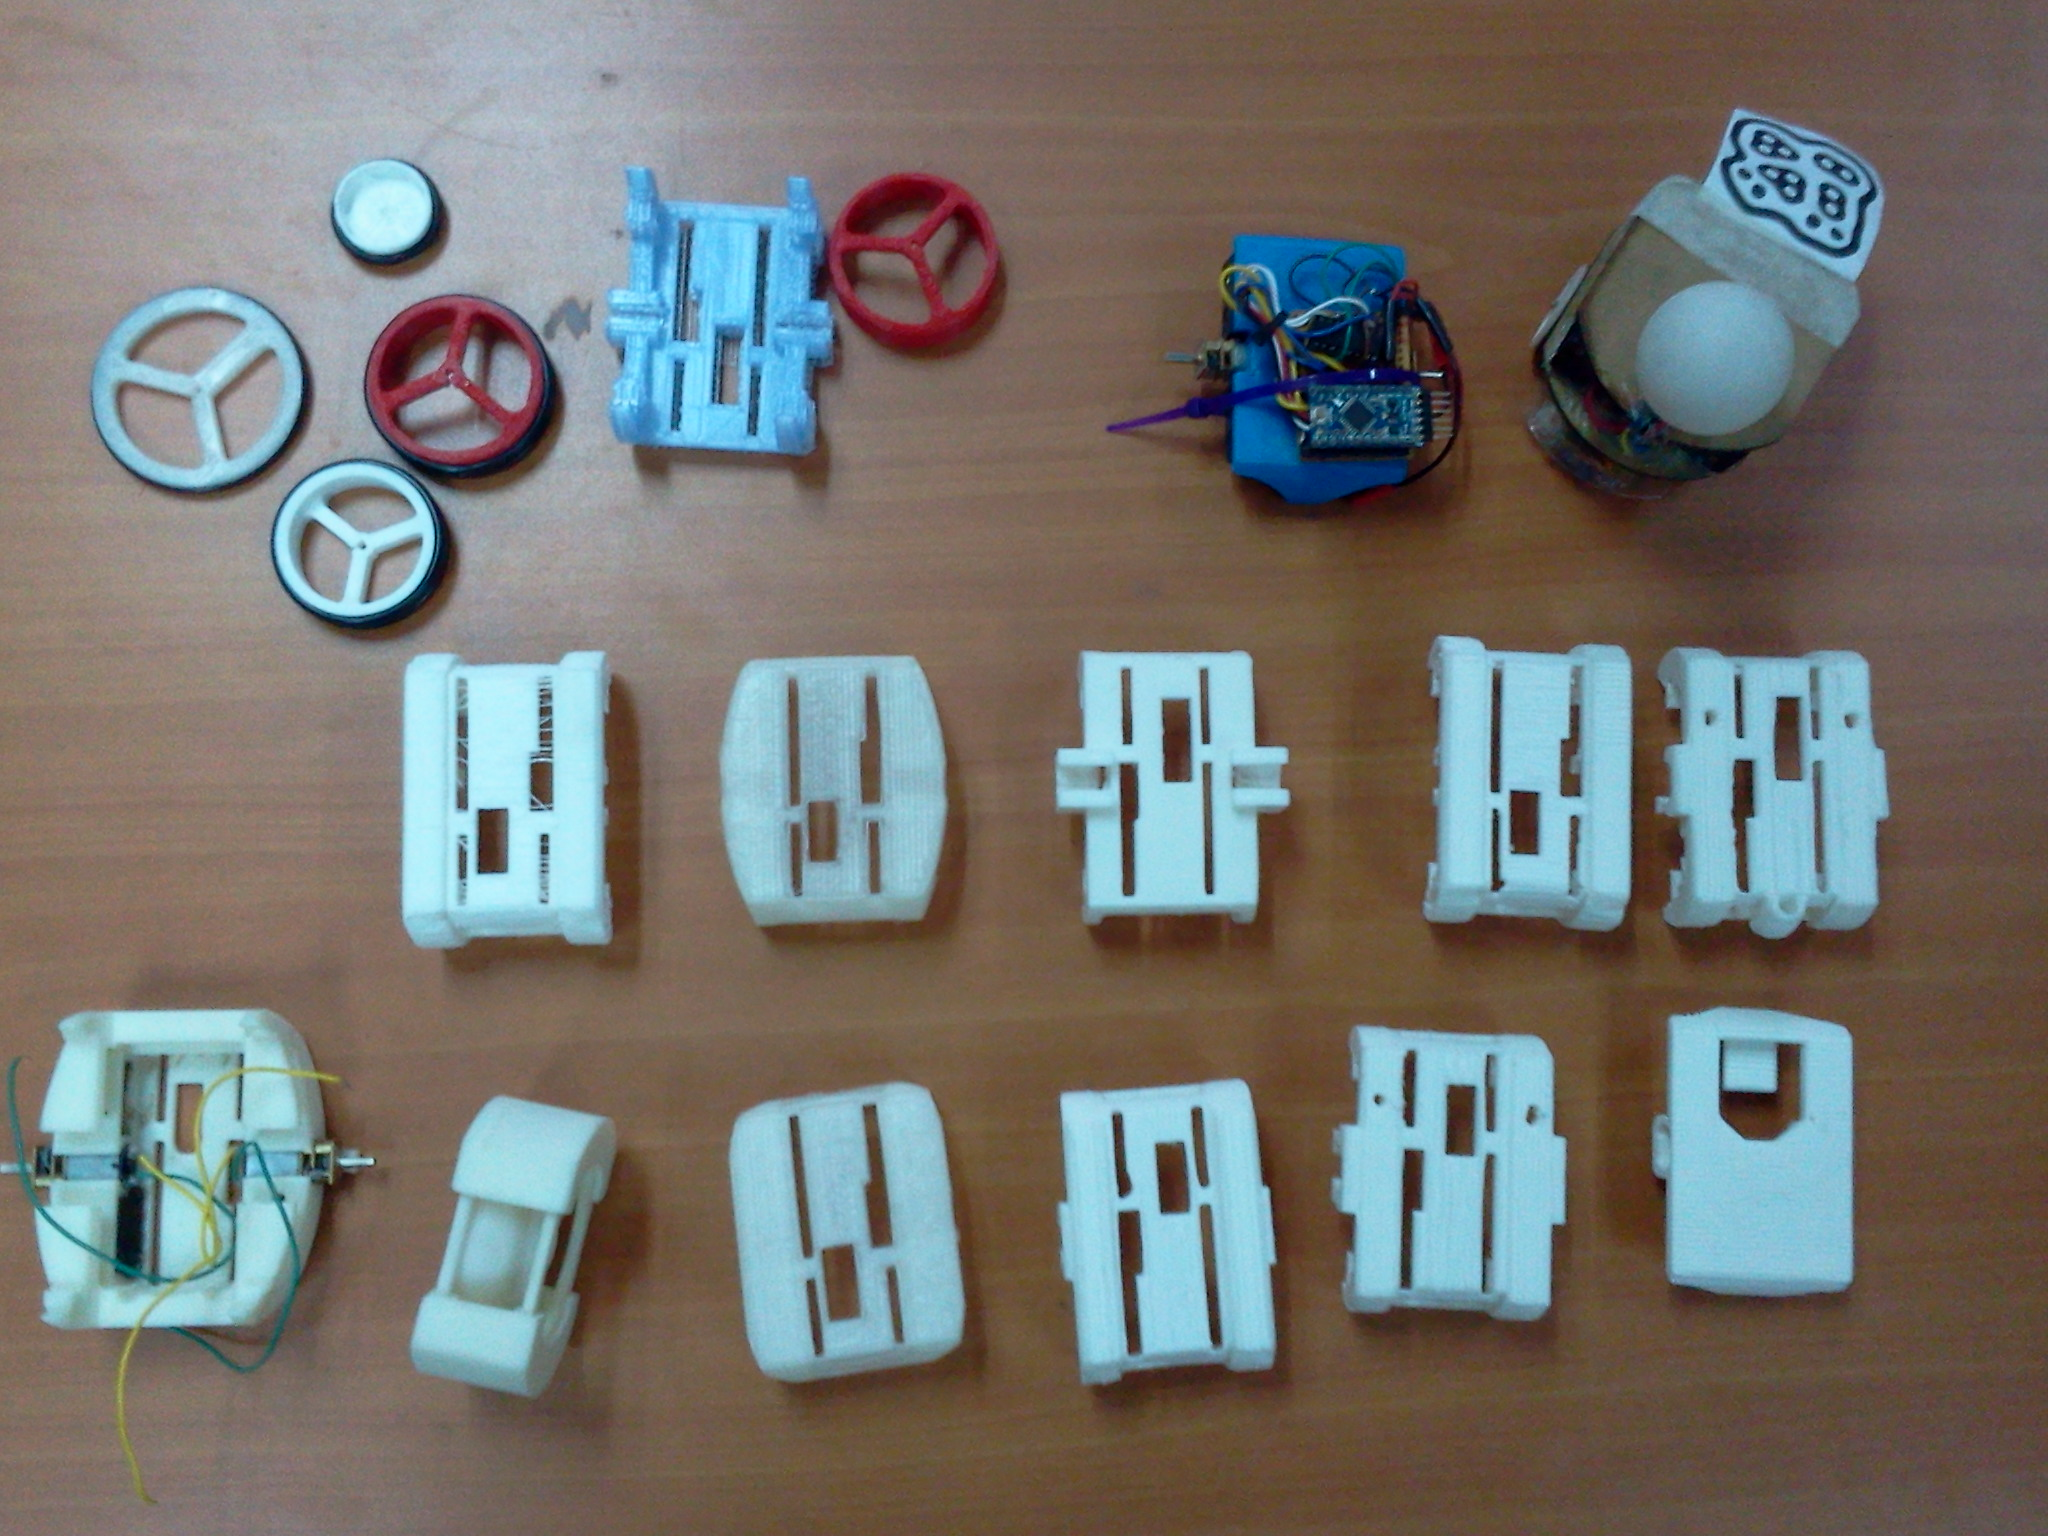
\includegraphics[width=\textwidth]{./Pictures/historia.jpg}
		\rule{35em}{0.5pt}
	\caption[Historia de construcción]{Algunos de los modelos que se construyeron para llegar a la versión final de MODI.}
	\label{fig:Historia}
\end{figure}

\newpage 
Lo segundo es el PCB diseñado para MODI que une el controlador de motores al arduino FIO y permite contectar un LED RGB.
\begin{figure}[htbp]
	\centering
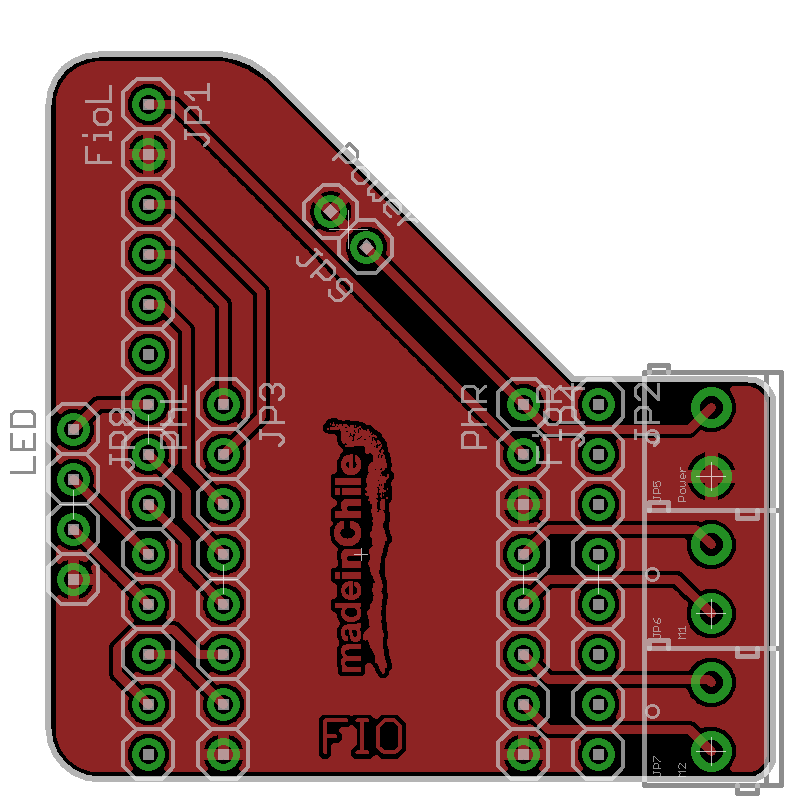
\includegraphics[width=\textwidth]{./Figures/MODI/pcbmodi.png}
		\rule{35em}{0.5pt}
	\caption[PCB MODI]{PCB diseñada para conectar motores, LED RGB al Arduino FIO.}
	\label{fig:Historia}
\end{figure}

%\input{./Appendices/AppendixB}
%\input{./Appendices/AppendixC}

\addtocontents{toc}{\vspace{2em}} % Add a gap in the Contents, for aesthetics

\backmatter

%----------------------------------------------------------------------------------------
%	BIBLIOGRAPHY
%----------------------------------------------------------------------------------------

\label{Bibliography}
%Renombrar pagina
\renewcommand{\bibname}{Referencias}
\renewcommand{\refname}{Referencias}

\lhead{\emph{Bibliography}} % Change the page header to say "Bibliography"

\bibliographystyle{unsrtnat} % Use the "unsrtnat" BibTeX style for formatting the Bibliography

\bibliography{Bibliography} % The references (bibliography) information are stored in the file named "Bibliography.bib"

\end{document}